\documentclass[letterpaper,journal]{IEEEtran}

\usepackage{amsmath,amsfonts,amssymb}
\usepackage{array}
\usepackage{url}
\usepackage{graphicx}
\usepackage{cite}
\usepackage{xcolor}
\usepackage{tikz}

\hyphenation{op-tical net-works semi-conduc-tor multi-modal token-izer token-izers}

\newcommand{\LAM}{large AI model}
\newcommand{\LAMs}{large AI models}
\newcommand{\GenAI}{generative AI}
\newcommand{\etal}{\emph{et al.}}
\newcommand{\etalspace}{\emph{et al.}\ }

\begin{document}

\title{From Generative to Embodied Intelligence: Network Evolution for Distributed Large-AI-Model Agents}

\author{Jihong Li, Bo Li,~\IEEEmembership{Student Member,~IEEE,}
Qingqing Wu,~\IEEEmembership{Senior Member,~IEEE,}
and Shunqing Zhang,~\IEEEmembership{Senior Member,~IEEE}%
\thanks{J. Li, B. Li, and S. Zhang are with the School of Communication and
Information Engineering, Shanghai University, Shanghai 200444, China.
Q. Wu is with the Department of Electronic Engineering, Shanghai Jiao Tong
University, Shanghai 200240, China. (Corresponding author: Shunqing Zhang.)}}

\markboth{IEEE Communications Surveys \& Tutorials,~Preprint}%
{Li \MakeLowercase{\textit{et al.}}: From Generative to Embodied Intelligence}

\maketitle

\begin{abstract}
Large AI models are evolving from generators that return digital content, to
agents that execute multi-step workflows, and further to embodied agents that
perceive, decide, and act in the physical world. This evolution changes the
volume, temporal structure, reliability target, and failure cost of network
traffic. A generative request tolerates elastic delivery if response quality is
preserved; an agentic workflow accumulates failure probability over tool calls;
and an embodied loop can become unsafe when multimodal observations or action
tokens are late, asynchronous, or distorted. This survey develops a
network-centric comparative framework across these three stages. It shows that
the same base network quantities---latency, rate, reliability, traffic density,
and connection density---remain relevant but increase by orders of magnitude,
while model-side emphasis moves from content fidelity, through end-to-end task
success, to closed-loop control and safety. It then traces architecture from
cloud-centric inference to stateful edge orchestration and hierarchical,
partially decentralized multi-agent control. Enabling technologies are mapped
to a token plane, a transport plane, and a coordination plane. A token-
recognition case study translates observable traffic and endpoint-declared
metadata into deployable service classes without requiring payload inspection.
Finally, the paper identifies tokenizer compatibility and incrementally
deployable token-aware protocols as prerequisites for networks that connect
distributed intelligence rather than merely transport bits.
\end{abstract}

\begin{IEEEkeywords}
Agentic AI, embodied AI, edge intelligence, large AI models, multi-agent
systems, networked control, semantic communications, token communications,
ultra-reliable low-latency communications.
\end{IEEEkeywords}

\section{Introduction}
\label{sec:introduction}
\IEEEPARstart{L}{arge} AI models are moving beyond a single prompt--response
exchange. Generative models synthesize text, images, audio, and video
\cite{nvidiagenai};
agentic models decompose goals, invoke tools, retrieve memory, and cooperate
with other models; embodied models close the loop between multimodal sensing
and physical actuation. We use \emph{\LAM} (LAM) as an umbrella term for these
foundation-model-based systems, including large language models (LLMs),
multimodal large language models (MLLMs), world models, and
vision--language--action (VLA) models. The three stages are not mutually
exclusive model families. Rather, they represent increasingly stringent
interaction contracts between intelligence, a network, and an environment.

Mobile and edge networks are therefore changing roles. In the generative
stage, a network primarily transports prompts, context, and output tokens to a
remote accelerator. In the agentic stage, it also binds tools, model context,
persistent memory, and multiple expert models into a reliable transaction.
In the embodied stage, the network becomes part of the plant: it carries
camera, depth, point-cloud, inertial, joint-state, and action streams whose age
and synchronization affect the next physical state. The ongoing 3GPP study on
6G use cases explicitly includes AI-agent communication and network-supported
AI/ML training and inference, illustrating this shift from generic
connectivity toward AI, data, and computing service exposure
\cite{3gpp22870}.

Prior work has largely examined the three stages in separate literatures.
Autoregressive language and text--image models established scalable token-based
generation \cite{gpt3,dalle}, while MMLU and BIG-bench broadened evaluation
beyond a single task \cite{mmlu,bigbench}. AgentBench evaluates tool-using
trajectories \cite{agentbench}, and ReAct and Reflexion study interleaved
reasoning, acting, feedback, and retry \cite{react,reflexion}. Embodied research
moves evaluation into manipulation and sensorimotor interaction through
Meta-World, RT-2, and LIBERO \cite{metaworld,rt2,libero}. In parallel,
communication-oriented studies cover mobile-edge LLM inference
\cite{edgeLLMsurvey}, semantic and token communications
\cite{semanticclassic,tokcom}, and integrated sensing and edge AI \cite{isea}.
These streams provide essential components, but use different units of
evaluation---content, task trajectory, and physical episode---which motivates a
cross-stage synthesis.

This transition exposes a mismatch between conventional communication
objectives and application value at every LAM stage. For a generative service,
average throughput does not reveal whether an interactive first token is late,
whether a variable-length multimodal response can be sustained, or whether the
delivered representation retains the required content quality. For an agentic
service, a stale tool result or one failed step can invalidate a long,
branching trajectory, while retries and growing memory make resource demand and
completion time highly variable. For an embodied service, a missing visual
patch may hide a grasp point and jitter may destabilize a fast control loop;
yet transporting every camera, range, joint-state, and action sample with
uniform fidelity is often infeasible. The central design question is therefore:
\emph{which information must be delivered, to which model or actuator, by
what deadline, and with what task-level loss when resources are limited?}

% \subsection{Positioning Relative to Adjacent Surveys}
% The topic is adjacent to, but broader than, several established survey areas.
% Edge-LLM studies primarily ask where a model should execute and how model,
% tensor, pipeline, or expert parallelism reduces inference cost. They usually
% treat the model output as the terminal objective. Semantic-communication
% studies replace bit fidelity with meaning or task fidelity, and recent token
% communication makes foundation-model tokens the exchanged representation
% \cite{semanticclassic,tokcom}. Integrated sensing and edge AI extends the
% objective to perception tasks and systematically co-designs sensing,
% communication, and inference \cite{isea}. URLLC and deterministic networking
% provide reliability and tail-delay tools, while wireless networked control
% directly optimizes stability, identification, or linear-quadratic cost.

% Each area solves one part of the embodied problem, but their boundary
% assumptions differ. Efficient LLM inference generally assumes that additional
% latency reduces user experience but not plant stability. Semantic
% communications commonly evaluates a reconstructed signal or a downstream
% classifier, for which occasional errors do not change the next source state.
% URLLC abstracts a packet source and deadline without asking which physical
% state generated the packet. Networked-control theory closes the loop but
% usually starts with an explicit low-dimensional dynamical model rather than a
% VLA policy and multimodal token stream.

% This survey uses model evolution to connect the areas. Its distinctive object
% is the \emph{distributed LAM agent service}: model execution, network
% transport, memory/tool interaction, and physical control are all parts of one
% service graph. Table~\ref{tab:positioning} makes the boundary explicit. The
% comparison is important because merely combining the mechanisms in adjacent
% columns does not ensure end-to-end validity. For example, a token-pruning
% method can preserve perception accuracy, and a URLLC link can deliver the
% retained tokens reliably, while the closed loop still fails because the
% pruned token marks a contact transition or the accelerator queue introduces
% jitter.

% \begin{table*}[t]
% \caption{Position of This Survey Relative to Adjacent Research Areas}
% \label{tab:positioning}
% \centering
% \footnotesize
% \renewcommand{\arraystretch}{1.17}
% \setlength{\tabcolsep}{3.1pt}
% \begin{tabular}{|p{0.15\textwidth}|p{0.18\textwidth}|p{0.18\textwidth}|p{0.18\textwidth}|p{0.21\textwidth}|}
% \hline
% \textbf{Area} & \textbf{Terminal objective} & \textbf{Traffic abstraction}
% & \textbf{Typical system boundary} & \textbf{What remains outside that
% boundary} \\ \hline
% Edge LLM inference &
% Inference latency, energy, accuracy, or cost &
% Requests, tensors, features, experts, and output tokens &
% Device--edge--cloud model serving &
% Tool transactions, control dynamics, task-dependent physical consequence
% \\ \hline
% Semantic/token communications &
% Semantic reconstruction or downstream inference quality &
% Meaning-bearing features or model tokens &
% Semantic encoder, channel, and semantic decoder &
% Long-horizon task dependency, actuator timing, and closed-loop stability
% \\ \hline
% Integrated sensing and edge AI &
% End sensing/perception task performance &
% Sensor signals and task-oriented features &
% Sensing--communication--edge inference &
% Agentic tools/memory and multi-rate action execution \\ \hline
% URLLC/deterministic networking &
% Packet error, hard deadline, delay tail, and jitter &
% Short packets and queues with service classes &
% Radio/access and sometimes edge-compute queue &
% Source semantics, cross-modal dependence, and physical-state evolution
% \\ \hline
% Wireless networked control &
% Stability, estimation/identification error, or control cost &
% State estimates, measurements, and control packets &
% Communication link plus an explicit dynamical plant/controller &
% Foundation-model uncertainty, tokenization, and implicit learned dynamics
% \\ \hline
% \textbf{This survey} &
% Content quality $\rightarrow$ task success $\rightarrow$ safe physical
% control &
% Tokens, transactions, multimodal observations, actions, and dependencies &
% Model--memory/tool--network--compute--physical service graph &
% Develops the interfaces and open problems needed to optimize the graph
% end-to-end \\ \hline
% \end{tabular}
% \end{table*}

\begin{figure*}[h]
\centering
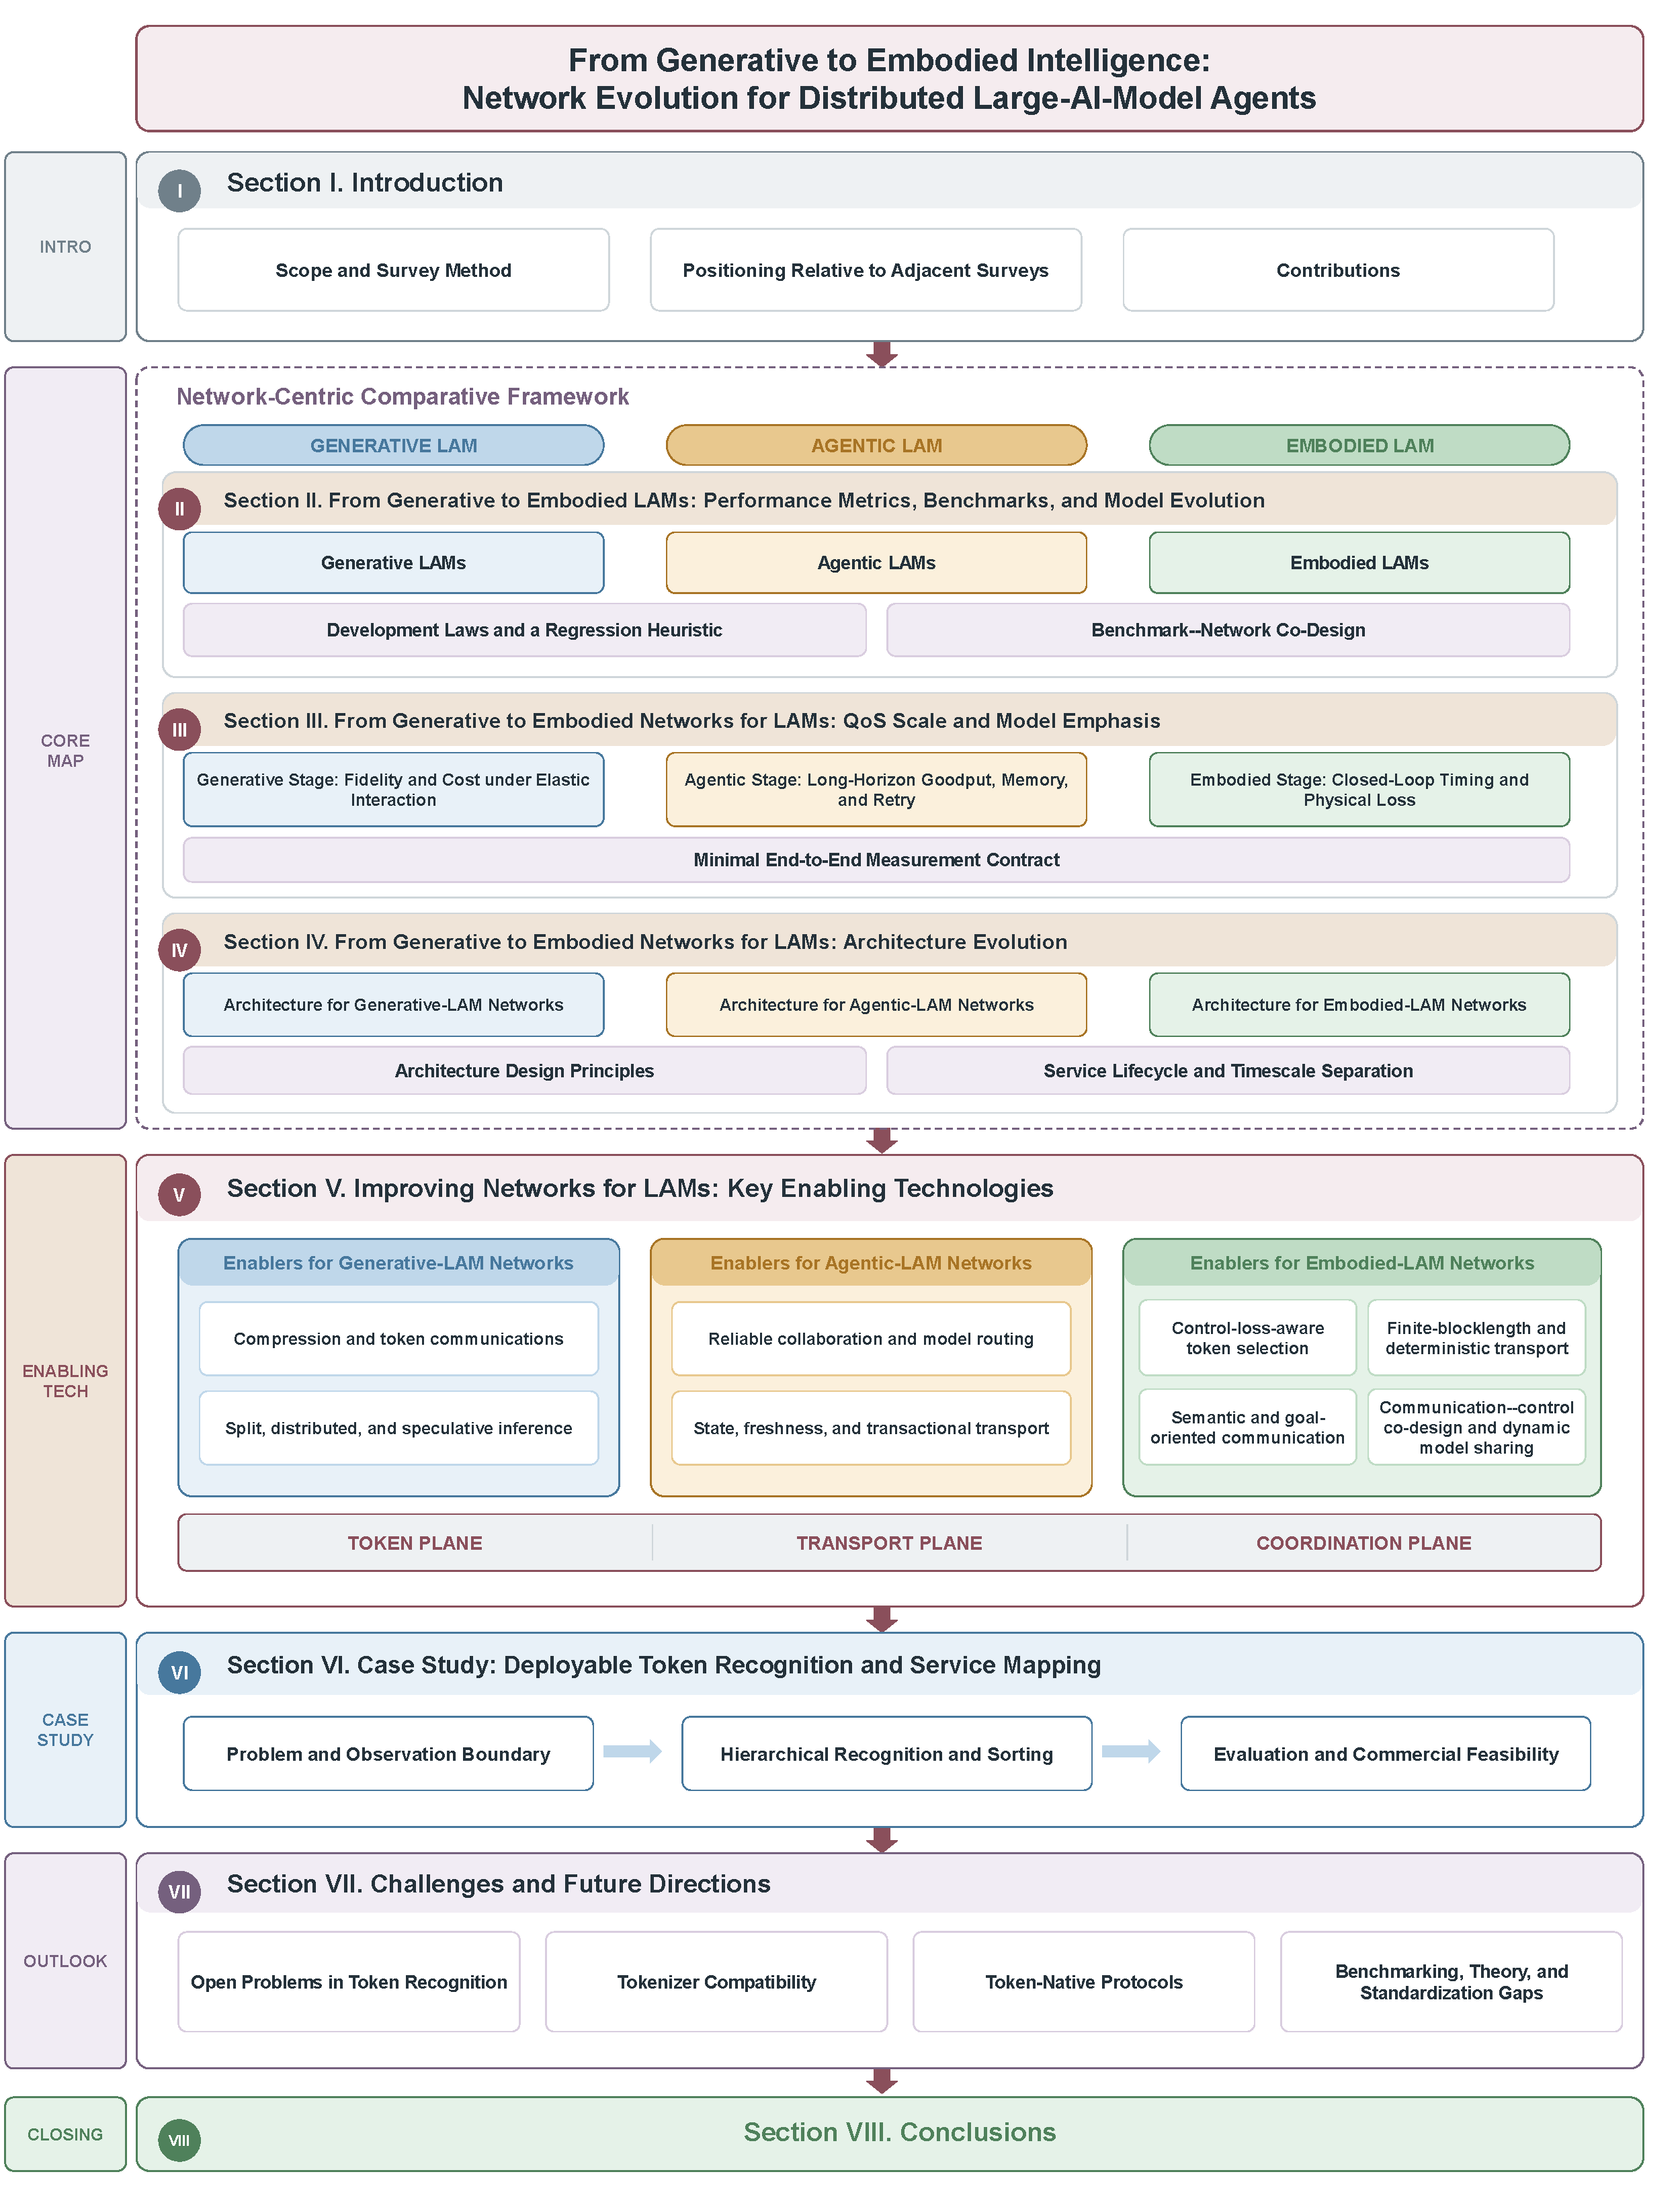
\includegraphics[width=0.75\linewidth, trim=0 0 0 0, clip]{Fig3_Survey_Roadmap.pdf}
\caption{The outline of this survey.}
\label{fig:roadmap}
\end{figure*}

\subsection{Contributions}
The survey makes four contributions.

\begin{itemize}
\item It synthesizes generative, agentic, and embodied systems through a
network-centric comparative framework that jointly classifies model objectives,
token sources, interaction patterns, benchmarks, failure consequences, and
network operating bottlenecks. 
% The contribution is the cross-stage mapping, not a claim that the three model categories are introduced here.
\item It maps AI-side evaluation to network-side quality of service (QoS).
The resulting metric ladder progresses from time to first token and content
quality, to transaction success and long-horizon tail latency, and finally to
task distortion, robust loop period, and control cost.
\item It organizes enabling technologies into token, transport, and
coordination planes and maps them back to the QoS and topology of each stage.
For embodied agents specifically, the synthesis exposes two transfer gaps:
compression is commonly perception-oriented rather than control-oriented, and
deterministic transmission is commonly source-independent rather than
task-coupled.
\item It develops a deployable token-recognition case study and derives
research directions for service classification, interoperability, and protocol
design under confidentiality and commercial-boundary constraints.
\end{itemize}

Section~\ref{sec:model_evolution} reviews model evolution and benchmarks.
Sections~\ref{sec:qos} and~\ref{sec:architecture} study metric and architecture
evolution, respectively. Section~\ref{sec:enablers} surveys enabling
technologies, Section~\ref{sec:case} presents the case study, and
Section~\ref{sec:future} discusses open challenges. The architecture of the main sections of the paper is presented in Fig.~\ref{fig:roadmap}. 

\section{From Generative to Embodied LAMs: Performance Metrics, Benchmarks, and Model Evolution}
\label{sec:model_evolution}
\subsection{Generative LAMs}
Generative LAMs learn a conditional distribution over token sequences
\cite{gpt3,dalle}.
Text is represented by subword tokens; images and video by spatial or
spatiotemporal patches or discrete latent codes; and audio by waveform,
spectral, or codec tokens. Transformer attention supplies a shared processing
interface, but it does not make these tokens computationally equivalent. A text
token may represent a word fragment, whereas a visual token represents a local
patch and an audio token represents a time interval.

Model-side evaluation in this stage is largely \emph{content-centric}.
Perplexity measures predictive fit \cite{gpt3}; exact-match or multiple-choice
accuracy measures knowledge and reasoning \cite{mmlu}; and BLEU and ROUGE
compare generated and reference text \cite{bleu,rouge}. MMLU spans 57 subjects
and tests broad academic knowledge \cite{mmlu}; BIG-bench uses more than 200
heterogeneous tasks to probe capabilities and scaling behavior
\cite{bigbench}. For open-ended and multimodal generation, human preference,
learned reward, semantic similarity, factuality, and safety are required because
literal word or phrase matching cannot capture meaning, visual quality, or
factual correctness.

The token workload depends strongly on both modality and direction. Text
understanding performs a parallel prefill over the prompt and retrieved
context, whereas text generation is autoregressive: it adds one token per
decoding step and grows the key--value cache with sequence length. Image
understanding processes a spatial patch grid \cite{vit}, while diffusion-based
image generation repeatedly evaluates a denoising model \cite{ddpm}. Video adds
a temporal token dimension to image processing, so its cost scales with frame
count as well as resolution; audio understanding and generation operate on
dense time-indexed spectral or codec tokens and often require causal streaming.
Consequently, long text output is dominated by sequential decoding, high-
resolution image synthesis by repeated denoising, and video generation by the
largest combined compute and memory footprint. These modality-dependent
workloads define the relevant local model characteristics in this section.

\subsection{Agentic LAMs}
An agentic LAM places a large AI model inside a feedback loop with a planner,
tool interfaces, memory, verification, and sometimes other agents
\cite{react,reflexion,du_debate}. The unit of work is no longer one output
sequence but a trajectory
\[
\tau=(o_0,a_0,o_1,a_1,\ldots,o_K),
\]
where observations $o_k$ may be web pages, application screenshots, database
results, code-execution logs, or messages from peer agents, and $a_k$ may call
an API or change external state. Reasoning techniques such as chain-of-thought
\cite{cot} and tree/graph search \cite{tot}, retrieval-augmented generation
\cite{rag}, model context protocols \cite{agentprotocols}, and multi-agent
debate \cite{du_debate} increase capability by introducing more rounds and
more state.

Consequently, evaluation shifts from answer similarity to
\emph{process-grounded task completion}. AgentBench, for example, evaluates
LLM agents across operating-system, database, knowledge-graph, gaming,
household, web-shopping, and web-browsing environments
\cite{agentbench}. WebArena tests goal completion in realistic websites
\cite{webarena}, whereas SWE-bench evaluates repository-level issue resolution
with executable tests \cite{swebench}. Across these benchmarks, relevant
metrics include task success rate, number of tool calls, constraint violations,
plan length, recovery from tool failure, long-horizon consistency, and cost per
completed task. An agent that produces fluent intermediate text but executes
the wrong transaction has failed.

Trajectory reliability compounds over the sequence. If step $k$ succeeds with
conditional probability $p_k$, a simplified serial workflow has
\begin{equation}
P_{\rm task}=\prod_{k=1}^{K}p_k,\qquad
P_{\rm fail}\leq\sum_{k=1}^{K}(1-p_k),
\label{eq:agent_reliability}
\end{equation}
where the equality assumes that each $p_k$ already conditions on prior
success. Even modest per-call error becomes material for large $K$.
The same trajectory exposes a model-side resource law. Let $L_k$ and $G_k$
denote the input-context and generated-token lengths at step $k$, let $n_k$
count branches or retries, and let ${\cal A}$ contain the concurrently live
branches. A useful accounting model is
\begin{equation}
\begin{split}
C_{\rm ag}&\simeq\sum_{k=1}^{K}n_k
\big[C_{\rm pre}(L_k)+C_{\rm dec}(L_k,G_k)\big],\\
M_{\rm KV}&=\Theta\!\left(N_{\rm layer}d
\sum_{j\in{\cal A}}L_j\right),
\end{split}
\label{eq:agent_resource}
\end{equation}
where $C_{\rm pre}$ and $C_{\rm dec}$ are prefill and decoding cost and $d$ is
the cached key/value width. Attention makes the prefill component grow
quadratically with context length, whereas the key--value cache grows linearly
with the live context \cite{vllm}. Tool outputs and retrieved memory increase
$L_k$ over the trajectory; branching and retry multiply both repeated prefill
and simultaneously resident caches. Agentic inference therefore combines
growing state, bursty local accelerator utilization, and a heavy-tailed total
compute demand rather than a single fixed-size decode.
Reason--act traces and verbal feedback enable exception handling and retry
\cite{react,reflexion}, but repeated attempts expand context, consume tokens,
and create a heavy tail in job completion time. Agentic-LAM evaluation should
therefore report the distribution of attempts, total model and tool calls,
recovery success, and terminal task outcome, rather than treating each call as
an independent prediction.

\subsection{Embodied LAMs}
Embodied LAMs ground language and vision in state estimation, world
prediction, planning, and action \cite{palme,rt2,dreamer3}. Architectures
include VLA models, latent
world models, bird's-eye-view transformers, and joint-embedding predictive
architectures. The observation $o_t$ can combine RGB/depth images, point
clouds, force/torque, inertial measurements, joint encoders, and messages from
other robots. The output $u_t$ can contain waypoints, discrete skills, joint
targets, or continuous control actions. Generalist humanoid models such as
GR00T N1 illustrate a trend toward shared representations across embodiments
and tasks \cite{groot}.

The benchmark moves into a physical or high-fidelity simulated loop.
Meta-World contains 50 manipulation tasks and evaluates multi-task
generalization \cite{metaworld}; RT-2 tests seen and unseen skills and semantic
generalization on real robots \cite{rt2}; and LIBERO measures knowledge
transfer across lifelong manipulation suites \cite{libero}. These widely used
benchmarks primarily score success or return under a benchmark-defined horizon
and do not standardize end-to-end inference latency. HumanoidBench includes
locomotion, stabilization, and whole-body manipulation and runs its
61-dimensional policy at 50~Hz \cite{humanoidbench}, while Habitat~3.0 adds
dynamic human collaborators and human-in-the-loop evaluation
\cite{habitat3}. ReflexBench directly exposes reaction time: its six dynamic
manipulation tasks sweep configurable latency under synchronous and
asynchronous inference \cite{reflexbench}. Accordingly, balance-sensitive,
non-stationary, and multi-actor evaluation should report task outcome jointly
with observation-to-action latency and effective control frequency, rather
than treating a fixed simulator step as evidence of real-time operation.
World models used for control are ultimately judged by episodic return and
planning quality, not merely reconstruction \cite{dreamer3}; a small
perception error may be harmless in one state but decisive near a contact
transition, so average token distortion alone is inadequate.

Embodied work uses task-specific objectives and reports task success, episodic
return, and trajectory or control error \cite{rt2,dreamer3,humanoidbench}. A
benchmark-specific finite-horizon control cost can be written as
\begin{equation}
J_{\rm c}=\mathbb{E}\!\left[\sum_{t=0}^{H}
\gamma^t\!\left(
\|x_t-x_t^\star\|_{\mathbf Q}^{2}
+\|u_t\|_{\mathbf R}^{2}
\right)\right],
\label{eq:control_cost}
\end{equation}
where $x_t$ is the physical state, $x_t^\star$ the task-dependent target,
$u_t$ the action, and $\mathbf Q$ and $\mathbf R$ weight state-tracking and
control effort. This is not proposed as a universal new score: each benchmark
must publish its horizon, weights, termination conditions, and component
metrics separately.

Embodied LAM workloads contain continuous, coupled perception and action
streams. The model must understand scene semantics, object relations, and task
intent from rich multimodal observations while updating actions in real time;
adding more frames or viewpoints improves grounding but increases token count
and inference cost. This creates a three-way local resource tension. Increasing
resolution, context length, or temporal history can improve scene and state
estimation, but consumes more operations and memory and lengthens
observation-to-action inference. Reducing precision, visual tokens, or action
updates saves compute and shortens latency, but can lower task accuracy or make
the controller miss a short transition. Increasing the update rate tightens
the per-cycle compute budget while repeating multimodal fusion more often.
These constraints are most severe in balance, contact-rich, and dynamic
multi-actor tasks; model evaluation should therefore report task accuracy or
return jointly with median and tail inference latency, effective control
frequency, peak memory, and energy on declared hardware.

\begin{table*}[t]
\caption{Model and Workload Evolution Across LAM Stages}
\label{tab:modeltaxonomy}
\centering
\footnotesize
\renewcommand{\arraystretch}{1.18}
\setlength{\tabcolsep}{3.2pt}
\begin{tabular}{|p{0.085\textwidth}|p{0.17\textwidth}|p{0.18\textwidth}|p{0.17\textwidth}|p{0.16\textwidth}|p{0.15\textwidth}|}
\hline
\textbf{Stage} & \textbf{Primary objective} & \textbf{Token/source structure}
& \textbf{Representative evaluation} & \textbf{Interaction/workload pattern}
& \textbf{Failure consequence} \\ \hline
Generative &
Produce useful and faithful digital content &
Subwords, image/video patches, audio or codec tokens; statistical and
cross-modal redundancy &
Perplexity, accuracy, MMLU, BIG-bench, BLEU/ROUGE, preference, factuality &
Prompt/context prefill followed by autoregressive decoding; modality-dependent
token count; one/few-shot interaction &
Hallucinated or degraded content; often detectable, retryable, and
non-physical \\ \hline
Agentic &
Complete a goal through reasoning, tools, memory, and collaboration &
Generated tokens plus UI frames, logs, API objects, retrieved memory, and
inter-agent messages; workflow-induced redundancy &
Task success, tool correctness, constraint violations, calls/steps, recovery,
cost per completed job &
Stateful multi-round graph with fan-out, retries, persistent context, and
long-tail completion time &
Wrong external operation or cascading plan failure; compensation may be
expensive or impossible \\ \hline
Embodied &
Perceive, predict, and act effectively in the physical world &
Multiview/multimodal perception, world-state and action tokens; spatial,
temporal, task, and physical coupling &
Task success, episodic return, action/trajectory error, world-model error,
planning quality, sim-to-real gap, control cost, inference latency &
Continuous, bidirectional, multisource loops at heterogeneous periods;
scene understanding and action updates at heterogeneous frequencies &
Task failure, unstable motion, or divergence from the commanded state; late
information can be worse than missing information \\ \hline
\end{tabular}
\end{table*}

\subsection{Development Laws and a Regression Heuristic}
Table~\ref{tab:modeltaxonomy} reveals four recurring development laws. 
\begin{itemize}
    \item Interaction frequency and coupling increase: a prompt is weakly coupled to the next request, an agent trajectory is logically coupled across steps, and an embodied trajectory is both logically and dynamically coupled through the environment.
    \item Failure propagates farther: a generative error usually affects one response, an agentic error can corrupt the remaining task graph and external state, and an embodied error changes the next observation through physical dynamics.
    \item The computational path evolves from one-pass generation, to iterative stateful trajectories, and then to continuous multi-rate perception--action loops. The dominant bottleneck consequently shifts from sequential decoding and key--value memory, to repeated inference and context expansion, and finally to concurrent multimodal fusion under a per-cycle deadline.
    \item The exploitable structure becomes richer: generative tokens mainly expose statistical redundancy, agentic trajectories add repeated context and workflow redundancy, and embodied streams add geometry-, kinematics-, and task-induced constraints. Selective computation and reuse therefore become more structured, but their validity must be judged at the response, trajectory, or closed-loop episode level.
\end{itemize}

An intuitive, but deliberately non-normative, interpretation is a
\emph{regression heuristic}. Artificial systems have scaled capabilities in an
order that is roughly opposite to the layering of human competence: codified
knowledge and content generation first, explicit planning and tool use next,
and robust sensorimotor interaction last. Conversely, loss of higher explicit
reasoning can leave basic procedural or reflexive behavior intact. The analogy
helps explain why generating fluent text does not imply reliable tool use, and
why either capability does not imply safe physical intelligence. It is neither
a biological law nor an originality claim; its engineering implication is only
that later stages inherit earlier representation and generation abilities while
adding state, timing, interaction, and physical grounding. And the embodied system requires more sophisticated training and ingenious system optimization. 

\subsection{Benchmark Design Across Stages}
Stressors must be injected at the model interface under study.
Generative evaluation should vary context length, output length, prompt
ambiguity, and modality corruption; agentic evaluation should inject tool
failure, stale or missing memory, and misleading intermediate observations;
embodied evaluation should vary viewpoint, occlusion, object layout, temporal
subsampling, and action noise. Temporal structure must be preserved: random
frame removal is not equivalent to losing a contiguous observation interval at
grasp contact.

The benchmark must also propagate a stressor to the terminal metric. For a
generative model this requires scoring the decoded output, not only an internal
feature error. For an agent it requires executing the remaining task graph,
because one wrong observation can alter later tool calls. For an embodied agent
it requires closing the physics loop; isolated perception accuracy cannot show
whether the resulting action succeeds safely.

The mapping also reveals a reproducibility hierarchy. A \emph{trace replay}
uses fixed model inputs and outputs and is inexpensive, but cannot represent
feedback. An \emph{interactive environment} executes tools or a simulator
against live model decisions. A \emph{hardware-in-the-loop} setup adds real
sensors or actuators and captures timing and embodiment effects. A
\emph{field trial} tests distribution shift and safety procedures.
Claims should match the highest validated level. In particular, a simulation
gain in task success is evidence for an orchestration principle, not proof of
real-world safety.

Finally, benchmark scores should be reported as a surface rather than a
single operating point. The surface relates model scale, token budget,
inference steps, compute load, and task quality. It exposes Pareto fronts
and phase transitions---for example, a stable range in which action reuse is
safe followed by a sharp loss near contact. Such a surface is the empirical
counterpart of the model and task tradeoffs that later system sections must
support.

\section{From Generative to Embodied Networks for LAMs: QoS Scale and Model Emphasis}
\label{sec:qos}

\begin{figure*}[h]
\centering
\setlength{\unitlength}{\linewidth}
\begin{picture}(1,0.2625)
\put(0,0){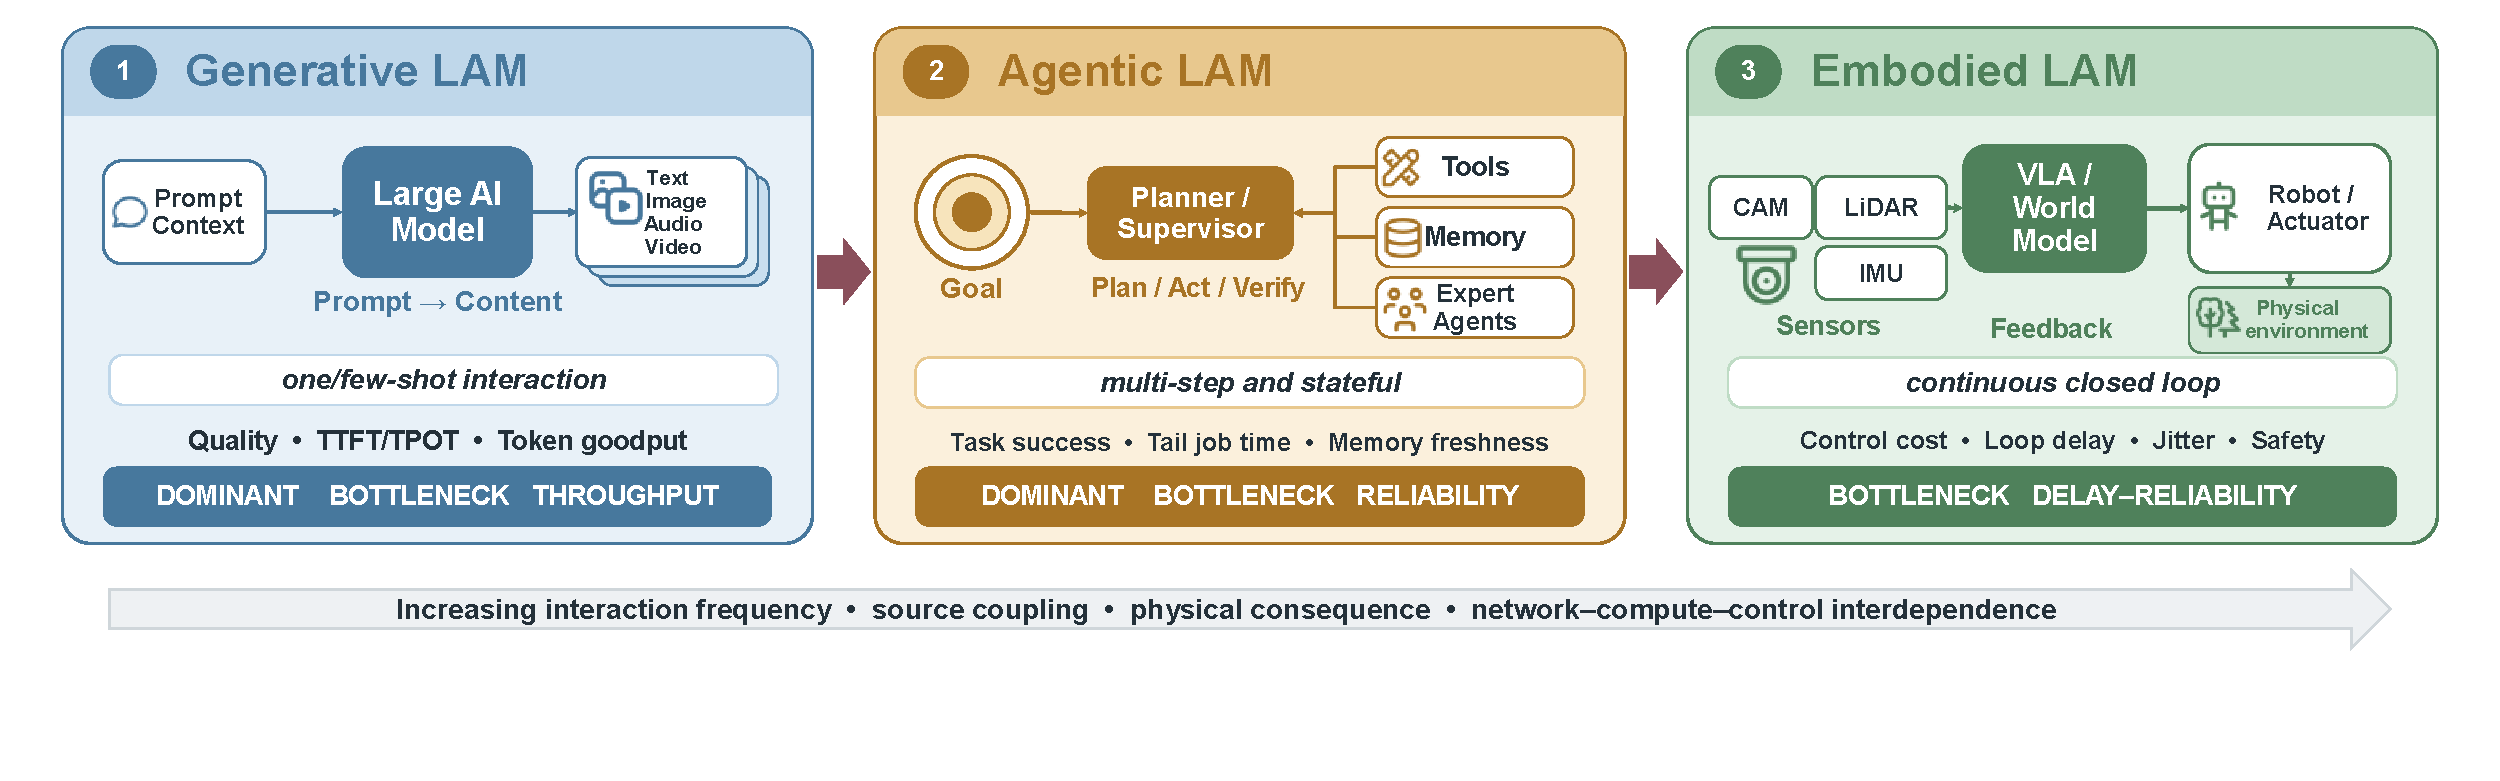
\includegraphics[width=\linewidth, trim=0 60 0 0, clip]{Fig1_LAM_Evolution.pdf}}
\put(0.476,0.205){\makebox(0,0){\color{black}\scriptsize$\circlearrowleft$ retry}}
\put(0.824,0.210){\makebox(0,0){\color{black}\scriptsize$\circlearrowleft$ 30 Hz}}
\end{picture}
\caption{Evolution of LAM services and their dominant network operating
bottlenecks. Requirements accumulate rather than replace one another:
embodied systems still need throughput and semantic reliability, but must
add deterministic closed-loop behavior. The circular marker on the
planner/supervisor denotes retry; each embodied sensing--action loop carries a
task-specific update rate, with 30 Hz shown as an illustrative requirement.}
\label{fig:evolution}
\end{figure*}

% \begin{figure*}[t]
% \centering
% \setlength{\tabcolsep}{2.5pt}
% \renewcommand{\arraystretch}{1.15}
% \begin{tabular}{c@{\hspace{4pt}$\Longrightarrow$\hspace{4pt}}c@{\hspace{4pt}$\Longrightarrow$\hspace{4pt}}c}
% \fbox{\parbox[c][1.08in][c]{0.275\textwidth}{\centering
% \textbf{Generative LAM}\\[2pt]
% Prompt $\rightarrow$ content\\
% one/few-shot interaction\\
% quality, TTFT, token goodput\\[2pt]
% \emph{dominant bottleneck: throughput}}}
% &
% \fbox{\parbox[c][1.08in][c]{0.275\textwidth}{\centering
% \textbf{Agentic LAM}\\[2pt]
% Goal $\rightarrow$ plan/tools/memory\\
% multi-step and stateful\\
% task success, tail job time\\[2pt]
% \emph{dominant bottleneck: reliability}}}
% &
% \fbox{\parbox[c][1.08in][c]{0.275\textwidth}{\centering
% \textbf{Embodied LAM}\\[2pt]
% Sense $\rightarrow$ predict $\rightarrow$ act\\
% continuous closed loop\\
% control cost, jitter, safety\\[2pt]
% \emph{bottleneck: delay--reliability}}}
% \\[5pt]
% \multicolumn{3}{c}{\small Increasing interaction frequency, source coupling,
% physical consequence, and network--compute--control interdependence}
% \end{tabular}
% \caption{Evolution of LAM services and their dominant network operating
% bottlenecks. Requirements accumulate rather than replace one another:
% embodied systems still need throughput and semantic reliability, but must
% add deterministic closed-loop behavior.}
% \label{fig:evolution}
% \end{figure*}

The three stages do not require three unrelated sets of network metrics.
Latency, bit and token rates, traffic and connection densities, reliability,
compute, storage, and energy remain the common engineering quantities. What
changes is primarily their \emph{order of magnitude} and the model-side loss
that qualifies delivered traffic as useful. Generative models emphasize
multimodal fidelity and decode efficiency; agentic models emphasize trajectory
success, retries, and long-term memory; embodied models emphasize synchronized
state estimation, control, and safety. Table~\ref{tab:qos}\footnote{Two cautions are essential. First, multiplying every maximum in one row by every maximum in another creates an impossible workload; duty factors and statistical multiplexing must be declared. Second, a ``token'' is not a fixed number of bits across text, images, video, latent states, or actions. Token rate therefore complements rather than replaces bit rate. The assumptions in Table~\ref{tab:qos} make sensitivity analysis possible: changing $r_0$,
$N_{\rm par}$, $L_{\rm state}$, $a$, or trajectory length $H$ immediately produces a new deployment-specific envelope.} gives a reproducible
scenario envelope that instantiates the radar-style comparison motivating this
survey. 
% The entries are design anchors, not standardized 6G requirements or simultaneous maxima.

\begin{table*}[t]
\caption{Order-of-Magnitude QoS Anchors and Explicit Scenario Basis}
\label{tab:qos}
\centering
\scriptsize
\renewcommand{\arraystretch}{1.17}
\setlength{\tabcolsep}{2.6pt}
\begin{tabular}{|p{0.16\textwidth}|p{0.095\textwidth}|p{0.095\textwidth}|p{0.095\textwidth}|p{0.445\textwidth}|}
\hline
\textbf{Common network quantity} & \textbf{Generative} &
\textbf{Agentic} & \textbf{Embodied} & \textbf{Interpretation/calculation
basis} \\ \hline
Network contribution to latency & $100$ ms & $10$ ms & $1$ ms &
Illustrative budget after separating model execution: interactive response,
multi-step coordination, and fast physical loop, respectively. Full
end-to-end latency still follows \eqref{eq:loop_delay}. \\ \hline
Peak service-token rate & $10^3$ token/s & $5\!\times\!10^4$ token/s &
$10^5$ token/s & $R_{\rm tok}=N_{\rm par}r_0$, with source-equivalent stream
rate $r_0=10^3$ token/s and parallel context/agent/modality counts
$N_{\rm par}=1,50,100$. \\ \hline
Peak service bit rate & $0.5$ Gbit/s & $5$ Gbit/s & $10$ Gbit/s &
A high-fidelity multimodal stream is the $0.5$-Gbit/s unit; agentic fan-out and
embodied multiview sensing aggregate roughly 10 and 20 such units. Compression
quality remains model- and modality-dependent \cite{evatok,edgeLLMsurvey}.
\\ \hline
Active-token density & $10^7$ token/km$^2$ & $10^8$ token/km$^2$ &
$10^9$ token/km$^2$ & $D_{\rm tok}=N_{\rm c}L_{\rm state}$ using
$L_{\rm state}=10^3$ active tokens per endpoint and the connection-density
anchors below. \\ \hline
Area traffic density & $10$ Tbit/s/km$^2$ & $100$ Tbit/s/km$^2$ &
$1000$ Tbit/s/km$^2$ & $D_b=10^{-3}N_{\rm c}ma r_b$, where $r_b$ is in
Gbit/s. The tuples $(m,a,r_b)$ are $(2,1,0.5)$, $(1,0.2,5)$, and
$(1,0.1,10)$; $m$ and $a$ denote parallel flows and active duty factor.
\\ \hline
Step/deadline reliability & $99\%$ & $99.9\%$ & $99.999\%$ &
$p_{\rm step}\ge P_{\rm task}^{1/H}$: $(P_{\rm task},H)=(0.99,1)$,
$(0.99,10)$, and $(0.999,100)$ yield approximately the listed anchors.
\\ \hline
Connection density & $10^4$/km$^2$ & $10^5$/km$^2$ & $10^6$/km$^2$ &
Tenfold scenario scaling from personal generative sessions, through dense
agent/tool endpoints, to massive sensors and physical agents; the top anchor
matches the established massive-connectivity order \cite{3gpp22870}. \\ \hline
\end{tabular}
\end{table*}

\begin{figure*}[t]
\centering
\definecolor{radargen}{RGB}{54,104,177}
\definecolor{radarag}{RGB}{230,126,34}
\definecolor{radaremb}{RGB}{39,145,96}
\begin{tikzpicture}[font=\scriptsize]
  % Concentric logarithmic-normalization guides.
  \foreach \r in {0.76,1.52,2.28,3.04}{
    \draw[gray!35] (90:\r)--(38.57:\r)--(-12.86:\r)--(-64.29:\r)--
      (-115.71:\r)--(-167.14:\r)--(141.43:\r)--cycle;
  }
  \foreach \a in {90,38.57,-12.86,-64.29,-115.71,-167.14,141.43}{
    \draw[gray!45] (0,0)--(\a:3.04);
  }
  \node[above,align=center] at (90:3.42) {Latency\\stringency};
  \node[right,align=left] at (38.57:3.45) {Peak service-\\token rate};
  \node[right,align=left] at (-12.86:3.42) {Peak service\\bit rate};
  \node[below right,align=left] at (-64.29:3.38) {Active-token\\density};
  \node[below left,align=right] at (-115.71:3.38) {Area traffic\\density};
  \node[left,align=right] at (-167.14:3.42) {Step/deadline\\reliability};
  \node[left,align=right] at (141.43:3.45) {Connection\\density};

  % Values are log-normalized from Table II; minima are displayed at 0.2.
  \draw[radargen,very thick,fill=radargen,fill opacity=0.09]
    (90:0.61)--(38.57:0.61)--(-12.86:0.61)--(-64.29:0.61)--
    (-115.71:0.61)--(-167.14:0.61)--(141.43:0.61)--cycle;
  \draw[radarag,very thick,fill=radarag,fill opacity=0.09]
    (90:1.82)--(38.57:2.67)--(-12.86:2.48)--(-64.29:1.82)--
    (-115.71:1.82)--(-167.14:1.42)--(141.43:1.82)--cycle;
  \draw[radaremb,very thick,fill=radaremb,fill opacity=0.07]
    (90:3.04)--(38.57:3.04)--(-12.86:3.04)--(-64.29:3.04)--
    (-115.71:3.04)--(-167.14:3.04)--(141.43:3.04)--cycle;

  \draw[radargen,very thick] (-2.95,-3.95)--(-2.45,-3.95)
    node[right,text=black] {Generative};
  \draw[radarag,very thick] (-0.55,-3.95)--(-0.05,-3.95)
    node[right,text=black] {Agentic};
  \draw[radaremb,very thick] (1.35,-3.95)--(1.85,-3.95)
    node[right,text=black] {Embodied};
\end{tikzpicture}
\caption{Radar view of the seven QoS anchors in Table~\ref{tab:qos}. Each
axis is logarithmically normalized between the smallest and largest tabulated
anchor; the minimum is plotted at 0.2 rather than the origin for visibility.
Latency and reliability increase outward as the latency budget and admissible
failure probability decrease. The polygons compare illustrative scenario
anchors, not standardized requirements or simultaneous maxima.}
\label{fig:qos_radar}
\end{figure*}

\subsection{Generative Stage: Fidelity and Cost under Elastic Interaction}
The content-centric benchmarks in Section~II first determine whether an output
is useful; service evaluation then adds time to first token (TTFT), time per
output token (TPOT), completion time, useful-token or bit goodput, and deadline
attainment. In the illustrative point in Table~\ref{tab:qos}, a generative
session combines a 100-ms network budget with $10^3$ token/s and a peak
0.5-Gbit/s multimodal flow. These quantities are strongly modality and request
dependent: interactive text tightens TTFT and token cadence, long outputs
extend the service interval, and high-fidelity image, audio, or video raises
the transient bit rate. The resulting numerical signature is therefore a wide
distribution of response sizes and completion times rather than one fixed-rate
flow, with content quality acting as the admissibility condition.

This signature burdens a current mobile network through variability and
burstiness. User arrivals can become correlated after a shared event, whereas
prompt length, output modality, and final response length are not fully known
at admission. Uplink prompts are followed by asymmetric downlink streams, and
short interactive sessions coexist with large media bursts. Conservative
reservation then wastes capacity between bursts, while best-effort scheduling
exposes TTFT and completion time to queueing tails. A generative-LAM network
should consequently characterize peak-to-mean load, burst duration, tail
queueing delay, and useful-token goodput in addition to average throughput.

\subsection{Agentic Stage: Long-Horizon Goodput, Memory, and Retry}
The process-grounded benchmarks in Section~II make the complete $K$-step task,
not an individual model response, the unit of success. Their task-success,
tool-correctness, attempts, recovery, and cost metrics translate into
end-to-end job time, per-step reliability, context freshness, active state,
and useful task-level goodput. For example, a 99\% target over ten serial steps
requires $p_{\rm step}\geq0.99^{1/10}=99.8995\%$, which motivates the 99.9\%
illustrative anchor in Table~\ref{tab:qos}. Its 10-ms network budget,
$5\!\times\!10^4$ token/s peak rate, and $10^5$/km$^2$ connection density
represent multiple concurrent agent, tool, memory, and verifier exchanges, not
a uniform rate sustained by every task. Longer plans and more branches tighten
the reliability requirement and broaden both state size and completion-time
distributions.

This numerical signature produces a different load on a mobile network. Task
graphs alternate silent tool execution with synchronized fan-out and fan-in;
timeouts, debate, and retries create microbursts, duplicate state, and a heavy
tail of unfinished jobs. The set of active flows changes during execution, so
admission and scheduling cannot rely on a fixed session graph or known payload.
Moreover, packet success is insufficient when an observation is stale, a tool
operation is duplicated, or a schema is inconsistent. The network must
therefore measure tail task-completion time, state freshness, retry-amplified
load, and completed-task goodput, while isolating correlated bursts from other
latency-sensitive services.

\subsection{Embodied Stage: Closed-Loop Timing and Physical Loss}
Embodied intelligence inherits generative fidelity and agentic trajectory
reliability, then adds sensing, actuation, and a physical deadline:
\begin{equation}
T_t^{\rm loop}=T_t^{\rm sense}+T_t^{\rm enc}+T_t^{\rm ul}
+T_t^{\rm queue}+T_t^{\rm inf}+T_t^{\rm dl}+T_t^{\rm act}.
\label{eq:loop_delay}
\end{equation}
Reducing radio time while increasing encoder or accelerator delay can worsen
the loop. For a loop period $h_i$, jitter tolerance $\epsilon_i$, and violation
probability $\delta_i$, a robust SLO is
\begin{equation}
\Pr\!\left\{T_{i,t}^{\rm loop}\le h_i,\,
\left|T_{i,t}^{\rm loop}-\mathbb{E}T_{i,t}^{\rm loop}\right|
\le\epsilon_i h_i\right\}\ge 1-\delta_i.
\label{eq:robust_slo}
\end{equation}
The first condition controls deadline reliability and the second jitter.
Asynchronous modalities also require age and skew bounds: a perfectly delivered
camera frame from before a contact transition can be less useful than a lower-
resolution but current frame.

For retained token set ${\cal K}$, goal $g$, and state $x$, define the
task-conditional distortion
\begin{equation}
D_{\rm task}({\cal K}\mid g,x)=J_{\rm c}({\cal K}\mid g,x)
-J_{\rm c}({\cal K}_{\rm full}\mid g,x).
\label{eq:task_distortion}
\end{equation}
The same token can be dispensable in free space and critical near an obstacle.
The corresponding economic metric should measure control improvement per total
resource cost:
\begin{equation}
\eta_{\rm EAI}=
\frac{J_{\rm c}^{\rm baseline}-J_{\rm c}^{\rm scheme}}
{\alpha B+\beta E+\chi F+\zeta S},
\label{eq:cost_effectiveness}
\end{equation}
where $B,E,F,S$ denote bandwidth, energy, compute cycles, and storage. This
form discourages spending large resources on tokens that do not improve the
physical task.

% \subsection{Minimal End-to-End Measurement Contract}
% The operator need not observe prompts, plans, sensor content, or actions. A
% commercially plausible contract keeps rich semantics inside the trusted
% endpoint/vertical and exposes only an authenticated service identifier,
% generation time, coarse deadline/reliability bin, chunk size, and an opaque
% causal identifier. Endpoint and compute-domain telemetry can privately bind the
% identifier to model queues and outcomes. Thus the carrier can attribute radio,
% path, and edge-queue delay without deep packet inspection or direct access to
% upper-layer state.

% Measurement granularity scales with risk: per-request aggregation for
% best-effort generation, per-step spans for an agentic transaction, and per-loop
% timing for an embodied service. Results should report percentiles and violation
% runs, condition on load, separate offered/decoded/useful goodput, and report
% joint freshness for fused modalities. For modalities $m\in{\cal M}_i$, a useful
% online proxy is
% \begin{equation}
% G_i^{\rm sync}=\frac{1}{|{\cal T}|}\sum_{k\in{\cal K}_i}
% v_k{\bf 1}\!\left\{t_k^{\rm rx}\le d_k,\,
% \max_{m,n\in{\cal M}_i}|a_m-a_n|\le s_i\right\},
% \label{eq:syncgoodput}
% \end{equation}
% where $v_k$ is an endpoint-assigned value bin, $a_m$ information age, and
% $s_i$ permitted skew. This metric is auditable network telemetry, not a
% replacement for application-owned quality or safety evaluation.

% The records close an assurance loop: admission predicts resource distributions,
% runtime monitoring detects joint violations, endpoints adapt compression,
% placement, or period, and aggregated outcomes update the next admission model.
% This limited exposure is sufficient for service-level engineering and is more
% deployable than assuming that a network can interpret raw tokens.

\section{From Generative to Embodied Networks for LAMs: Architecture Evolution}
\label{sec:architecture}

Architecture evolves along three coupled axes: \emph{placement} across device,
edge, and cloud; \emph{network topology} among models, users, tools, and
sensors; and \emph{collaboration mode} among agents. Centralization is not a
binary choice. One-to-one offloading, many-to-one aggregation, one-to-many
dispatch, peer-to-peer exchange, and hierarchical hybrids coexist and should be
selected by task dependency, latency, trust, and physical coupling.

\subsection{Architecture for Generative-LAM Networks}
A generative-LAM network is commonly cloud-centric. User equipment performs
tokenization and lightweight preprocessing; an edge gateway provides
admission, caching, privacy filtering, or small-model inference; and a cloud
cluster hosts the full model. Model, tensor, pipeline, and expert parallelism
distribute inference inside or across clusters. Wireless distributed
mixture-of-experts systems additionally make expert routing dependent on
channel and compute heterogeneity \cite{wdmoe}. Pipeline parallelism and
batching trade communication bubbles against accelerator utilization
\cite{pipeline}.

The dominant topology is one-to-one user--model access over a many-to-one
serving hub. Users collaborate indirectly by sharing batches, model replicas,
and KV-cache infrastructure, rather than by exchanging task state. The edge
absorbs latency-sensitive or private work and the cloud supplies model scale;
this cloud--edge--device continuum is the basic mobile-edge-intelligence
architecture for LLMs \cite{edgeLLMsurvey}.

The main control loop is a slow resource-management loop: predict request and
token lengths, place models, reserve accelerators and backhaul, batch
compatible requests, and route overflow. Split inference places early layers
on the device and later layers at the edge, transmitting intermediate
features. Progressive feature transmission allows a receiver to stop once
confidence is sufficient \cite{progressive}. This architecture is effective
when the user transaction is largely independent and deadlines are elastic.
It becomes inefficient when every intermediate action depends on fresh tool
or environment state.

\subsection{Architecture for Agentic-LAM Networks}
Agentic architecture adds a stateful orchestration plane. A planner or
supervisor discovers capabilities, selects models and tools, maintains a task
graph, and commits results to short- and long-term memory. Executors can be
distributed over devices, edge sites, enterprise services, and clouds.
Messages carry not only tokens but role, goal, schema, provenance, confidence,
and dependency. Multi-agent systems use debate, vote, expert routing, or
hierarchical decomposition; the best topology depends on task structure and
the correlation of model errors \cite{agentsmobile,du_debate,estornell}.
One-to-many dispatch appears when a planner fans out to tools or specialists;
many-to-one aggregation appears in voting and fusion; peer-to-peer exchange
supports decentralized debate; and a supervisor plus peer subgraphs forms a
hybrid. Emerging MCP, ACP, A2A, and ANP families cover different discovery,
tool-access, messaging, and decentralization assumptions
\cite{agentprotocols}. Thought- or latent-state exchange may further change the
payload while retaining the same task graph \cite{thoughtcomm,latentcomm}.

This design resembles a distributed transaction system but has probabilistic
components. It requires:
\begin{enumerate}
\item capability and context discovery before routing;
\item session affinity for key--value caches and private memory;
\item checkpoint, retry, and idempotence semantics for tool calls;
\item verification paths for high-impact actions; and
\item joint compute--network--storage admission for the complete task rather
than each RPC.
\end{enumerate}
The architecture may keep a small model on-device for privacy and rapid
screening, escalate uncertain inputs to a remote large model, and invoke
specialists only when their expected information gain exceeds their latency
and cost. Uncertainty-aware hybrid inference is one realization of this
principle \cite{hybrid}.

\subsection{Architecture for Embodied-LAM Networks}
Embodied systems require a hierarchy of loops (Fig.~\ref{fig:architecture}).
A local reflex/control plane executes high-rate stabilization and safety
interlocks. An edge cognition plane performs multimodal fusion, VLA inference,
local mapping, and coordination with deterministic access. A cloud learning
plane provides large-model reasoning, fleet memory, simulation, and
non-real-time model updates. A slow cloud model should not directly occupy a
hard real-time loop; it supplies goals, policies, latent plans, or verified
skill updates to an edge/local controller. Decentralized local safety and
reflexes coexist with temporarily centralized edge fusion. Consequently,
collaboration becomes dynamic and partially centralized rather than globally
centralized or fully peer-to-peer.

\begin{figure*}[t]
\centering
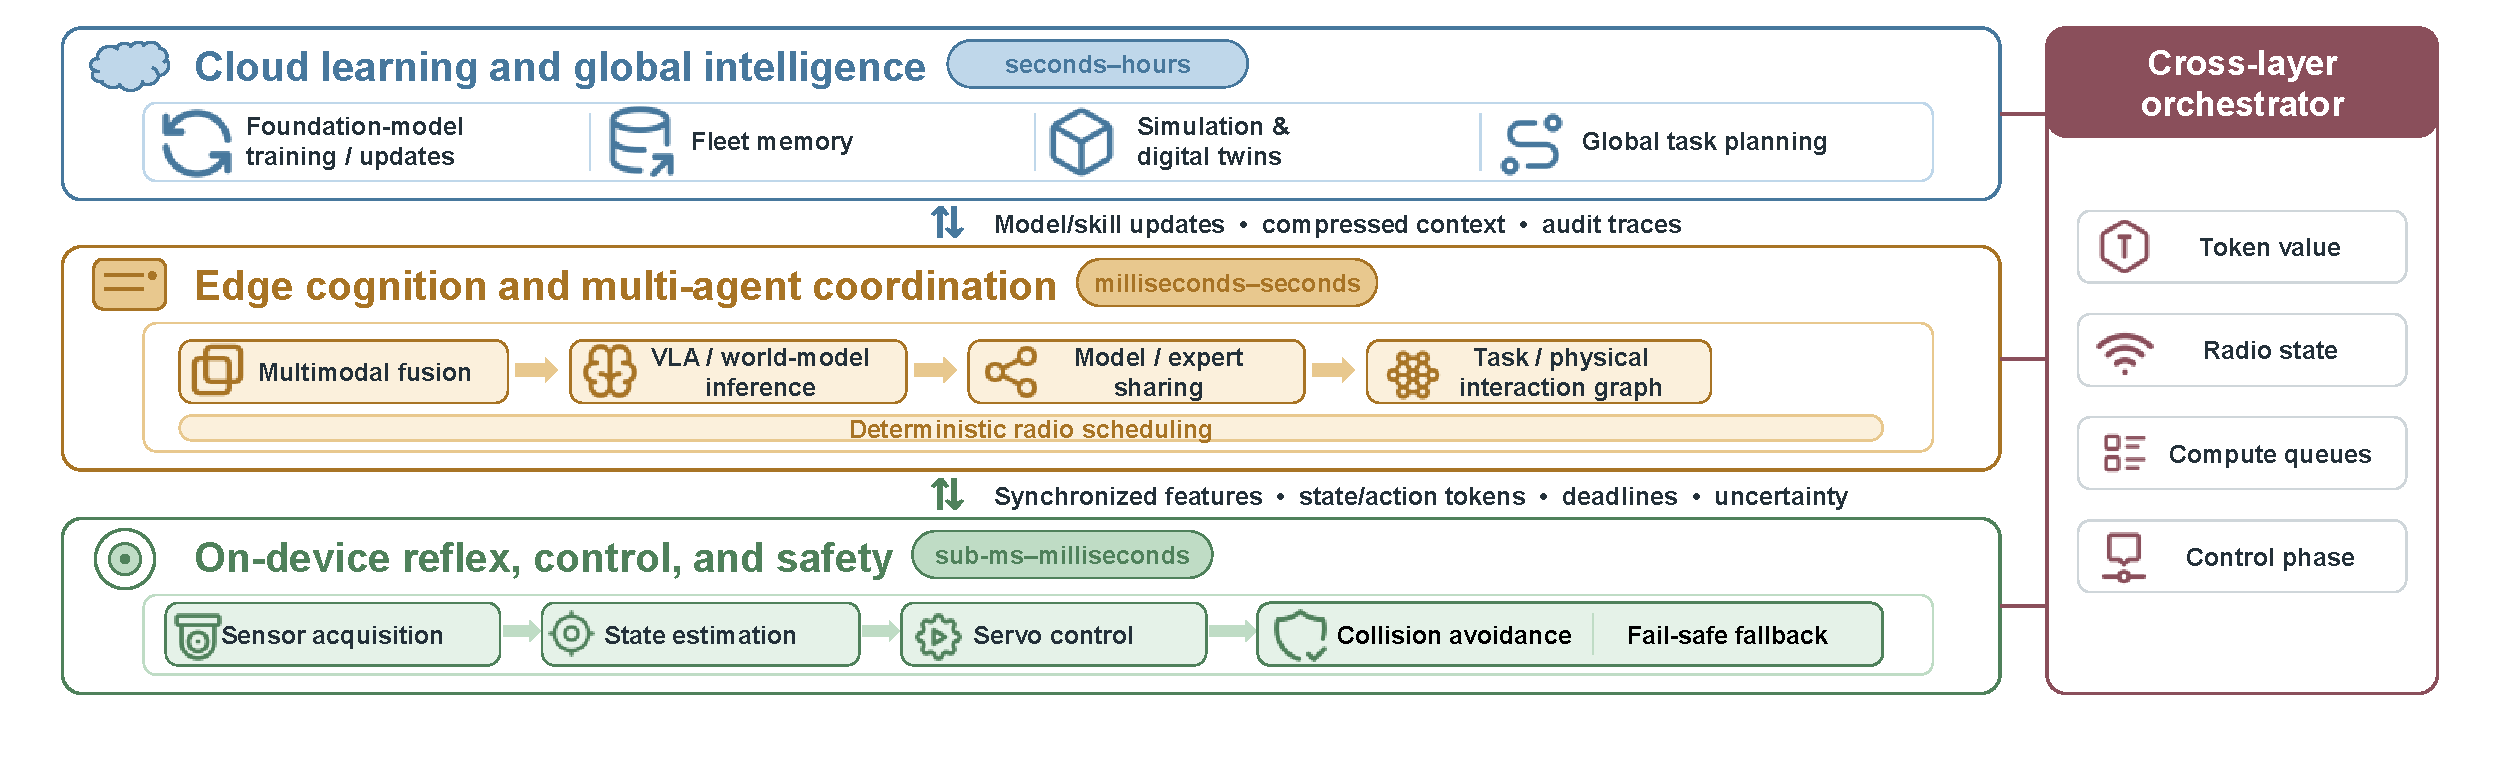
\includegraphics[width=\linewidth, trim=0 40 0 0, clip]{Fig2_LAM_Architecture.pdf}
\caption{Cloud--edge--device hierarchy for distributed LAM services. The
generative stage primarily uses cloud scale, the agentic stage adds stateful
edge orchestration, and the embodied stage keeps hard safety and stabilization
local while the edge closes latency-critical cognition and coordination loops.}
\label{fig:architecture}
\end{figure*}

% \begin{figure*}[t]
% \centering
% \setlength{\tabcolsep}{3pt}
% \renewcommand{\arraystretch}{1.2}
% \begin{tabular}{c}
% \fbox{\parbox{0.88\textwidth}{\centering
% \textbf{Cloud learning and global intelligence (seconds--hours)}\\
% foundation-model training/updates $\mid$ fleet memory $\mid$ simulation and
% digital twins $\mid$ global task planning}}\\[-1pt]
% $\Updownarrow$ \small model/skill updates, compressed context, audit traces\\[-1pt]
% \fbox{\parbox{0.88\textwidth}{\centering
% \textbf{Edge cognition and multi-agent coordination (milliseconds--seconds)}\\
% multimodal fusion $\mid$ VLA/world-model inference $\mid$ model/expert sharing
% $\mid$ task/physical interaction graph $\mid$ deterministic radio scheduling}}\\[-1pt]
% $\Updownarrow$ \small synchronized features, state/action tokens, deadlines,
% uncertainty\\[-1pt]
% \fbox{\parbox{0.88\textwidth}{\centering
% \textbf{On-device reflex, control, and safety (sub-ms--milliseconds)}\\
% sensor acquisition $\mid$ state estimation $\mid$ servo control $\mid$
% collision avoidance $\mid$ fail-safe fallback}}\\[3pt]
% \multicolumn{1}{c}{\small
% \textit{Cross-layer orchestrator: token value + radio state + compute queues +
% control phase}}
% \end{tabular}
% \caption{Cloud--edge--device hierarchy for distributed LAM services. The
% generative stage primarily uses cloud scale, the agentic stage adds stateful
% edge orchestration, and the embodied stage keeps hard safety and stabilization
% local while the edge closes latency-critical cognition and coordination loops.}
% \label{fig:architecture}
% \end{figure*}

The architecture is also \emph{partially centralized}. If two robots have
neither task dependence nor physical interference, merging their observations
in one model can add quadratic attention cost without useful information.
When they jointly carry an object or occupy the same collision region,
shared inference can improve consistency and reduce duplicated sensing. Let
${\cal G}_t=({\cal V},{\cal E}_t)$ be a time-varying interaction graph with
\begin{equation}
w_{ij}(t)=\rho_{\rm task} I_{ij}^{\rm task}(t)
+\rho_{\rm phy} I_{ij}^{\rm phy}(t)
+\rho_{\rm info} I_{ij}^{\rm info}(t),
\label{eq:interaction}
\end{equation}
where the three terms quantify task dependency, physical interference, and
complementary information. Clustering or sparsifying ${\cal G}_t$ determines
which agents share a model or exchange tokens. The resulting groups can run
at different loop periods, producing an asynchronous, multi-rate networked
control system.

\begin{table*}[t]
\caption{Placement, Networking Topology, and Collaboration Evolution}
\label{tab:architecture}
\centering
\footnotesize
\renewcommand{\arraystretch}{1.18}
\setlength{\tabcolsep}{3pt}
\begin{tabular}{|p{0.08\textwidth}|p{0.175\textwidth}|p{0.19\textwidth}|p{0.185\textwidth}|p{0.20\textwidth}|p{0.085\textwidth}|}
\hline
\textbf{Stage} & \textbf{Cloud--edge--device placement} &
\textbf{Typical topology} & \textbf{Collaboration law} &
\textbf{Persistent state/coupling} & \textbf{Timescale} \\ \hline
Generative &
Device front end; edge gateway/cache or small model; cloud accelerator cluster
& One-to-one request path over a many-to-one serving/cache hub; occasional
split pipeline & Resource sharing dominates direct agent cooperation:
admission, batching, cache-aware routing, and expert placement & Request,
model/tokenizer version, KV cache, queue and radio--compute utilization &
Request and decode \\ \hline
Agentic &
Device supervisor; edge session/state broker; distributed cloud/edge models,
tools, and stores & One-to-many planner dispatch, many-to-one vote/fusion,
peer debate, or supervisor--peer hybrid & Collaboration follows the task graph;
central orchestration gives way to decentralized/hybrid execution when trust,
failure isolation, or scale requires it & Goal, dependencies, memory/context
version, tool side effects, provenance; network--compute--storage transaction &
Step and workflow \\ \hline
Embodied &
Local reflex/safety; edge VLA/world-model fusion; cloud fleet learning and
simulation & Dynamic many-to-many interaction graph with local peer links and
temporary edge-centered clusters & Partial centralization follows task and
physical coupling; local safety persists while shared inference is activated
only for interacting agents & Multimodal time/age, action history, uncertainty,
safety envelope; sensing--communication--computing--control coupling &
Sub-ms--hours \\ \hline
\end{tabular}
\end{table*}

\subsection{Architecture Design Principles}
Three principles follow. First, \emph{place deadlines before models}: determine
which loop can tolerate cloud, edge, or only local execution before selecting
model size. Second, \emph{centralize only useful mutual information}: shared
models should be activated by task or physical coupling rather than by agent
density alone. Third, \emph{retain a safe degraded mode}: if the edge model,
radio link, or clock synchronization fails, the device must fall back to a
local controller that maintains a safe set, even if task progress stops.

% \subsection{Service Lifecycle and Timescale Separation}
% Architecture must cover the service lifecycle, not only the inference data
% path. During
% \emph{registration}, an endpoint or vertical gateway publishes an authenticated
% coarse capability/SLO manifest; detailed model state, sensor content, action
% semantics, and safety policy remain inside its trust domain. During
% \emph{admission}, the orchestrator maps a requested service
% to a service graph, predicts complete resource demand, selects placements,
% and rejects or degrades a task whose robust SLO is infeasible. During
% \emph{execution}, fast schedulers allocate token, radio, and compute resources
% under the admitted envelope. During \emph{recovery}, endpoints switch models,
% paths, or controllers and preserve transaction semantics. During
% \emph{learning}, traces update workload, token-value, channel, and physical
% interaction models.

% % \begin{figure*}[t]
% % \centering
% % \setlength{\tabcolsep}{2.2pt}
% % \renewcommand{\arraystretch}{1.05}
% % \begin{tabular}{c@{\,$\rightarrow$\,}c@{\,$\rightarrow$\,}c@{\,$\rightarrow$\,}c@{\,$\rightarrow$\,}c}
% % \fbox{\parbox[c][0.78in][c]{0.15\textwidth}{\centering\textbf{Register}\\
% % capability\\version/trust\\fallback}}
% % &
% % \fbox{\parbox[c][0.78in][c]{0.15\textwidth}{\centering\textbf{Admit}\\
% % service graph\\placement\\risk budget}}
% % &
% % \fbox{\parbox[c][0.78in][c]{0.15\textwidth}{\centering\textbf{Execute}\\
% % token value\\radio/compute\\loop monitor}}
% % &
% % \fbox{\parbox[c][0.78in][c]{0.15\textwidth}{\centering\textbf{Recover}\\
% % reroute/retry\\safe mode\\rollback}}
% % &
% % \fbox{\parbox[c][0.78in][c]{0.15\textwidth}{\centering\textbf{Learn}\\
% % causal trace\\model update\\SLO revision}}
% % \\[-1pt]
% % \multicolumn{5}{c}{\small
% % $\longleftarrow$ aggregated outcomes and revised workload/risk envelopes feed
% % the next registration and admission cycle $\longleftarrow$}
% % \end{tabular}
% % \caption{Closed assurance loop for a distributed LAM-agent service. Execution
% % is only one stage; versioned registration and admission bound runtime risk,
% % while recovery and privacy-preserving outcome feedback revise the next cycle.}
% % \label{fig:lifecycle}
% % \end{figure*}

% The lifecycle contains at least three control timescales.
% \begin{itemize}
% \item At a \emph{planning timescale} (minutes to hours), models and adapters
% are placed, capacity and slices are reserved, and fleet-wide policies are
% updated. Forecast error dominates.
% \item At a \emph{task timescale} (hundreds of milliseconds to minutes),
% agents/tools are selected, model-sharing groups and loop periods change, and
% context migrates. Task and physical topology dominate.
% \item At a \emph{loop/slot timescale} (sub-millisecond to tens of
% milliseconds), features and actions are scheduled, short packets are coded,
% and compute slots are aligned. Channel, queue, and release-time uncertainty
% dominate.
% \end{itemize}
% Optimizing every variable at the fastest timescale is neither feasible nor
% stable. Slow decisions should pass resource and risk budgets downward; fast
% controllers should return feasibility margins and violation statistics.
% When fast scheduling cannot maintain an admitted envelope, it should trigger
% a defined degradation---smaller model, fewer views, slower noncritical loop,
% or local safe mode---rather than silently accumulating queue.

% Mobility makes state migration a first-class operation. A generative session
% can move after transferring a key--value cache, subject to a short pause. An
% agentic session also needs memory and tool-transaction state. An embodied
% session cannot pause an unsafe plant while a large cache migrates. Predictive
% handover should replicate only the state needed to continue the near-term
% loop, keep stabilization local, and transfer large context in the background.
% Multi-tier computation offloading \cite{multitier} and ultra-low-latency edge
% inference \cite{edgeinference}, together with reliability-aware edge
% offloading \cite{offloading}, provide resource-allocation foundations, but
% embodied migration adds continuity of action and safety state.

% Finally, administrative and physical trust domains need not coincide. A
% warehouse owner, robot vendor, network operator, and cloud-model provider may
% control different lifecycle stages. The architecture therefore needs signed
% capability manifests, explicit data-use policy, model provenance, and
% auditable responsibility at every boundary. The vertical remains responsible
% for translating private semantics and safety policy into coarse service
% classes; the operator authenticates, meters, and polices those classes without
% requiring raw-token visibility.

\section{Improving Networks for LAMs: Key Enabling Technologies}
\label{sec:enablers}

We group mechanisms into three interacting planes. The \emph{token plane}
decides what representation to compute and communicate. The
\emph{transport plane} decides how to deliver it by a deadline. The
\emph{coordination plane} decides which agents/models should share
information and how network and compute resources close the loop. These planes
are not a separate taxonomy: Table~\ref{tab:stageenablers} maps each one to the
common QoS scale in Table~\ref{tab:qos} and the placement/topology in
Table~\ref{tab:architecture}.

\subsection{Enablers for Generative-LAM Networks}
\subsubsection{Compression and token communications}
Quantization, structured pruning, low-rank adaptation, key--value-cache
compression, and top-$k$/top-$p$ decoding reduce memory, computation, or
output entropy. Token communications elevates tokens to semantic
communication units and uses cross-modal context to reconstruct masked or
corrupted content \cite{tokcom}. Compared with conventional source coding, a
receiver equipped with a compatible foundation model can exploit learned
priors. This can reduce payload but transfers burden to shared model state,
tokenizer agreement, uncertainty calibration, and semantic error detection.
For video generation, EVATok adapts sequence length to the content and exposes
an explicit tradeoff between token count and reconstruction/generation quality
\cite{evatok}.
Token-domain multiple access further lets many devices share tokenizer and
modulation codebooks, using contextual reconstruction to mitigate token
collisions \cite{todma}. It targets the high token and connection densities in
Table~\ref{tab:qos}, but its gains depend on codebook compatibility and on
whether reconstructed content satisfies the generative quality target.

For sources $Z_1,\ldots,Z_M$ and task goal $g$, the relevant multi-source
rate--distortion function is conceptually
\begin{equation}
\begin{split}
R_g(D)&=\min_{p(\hat z|z_1,\ldots,z_M)}
I(Z_1,\ldots,Z_M;\hat Z\mid g),\\[-2pt]
&\hspace{8pt}\text{s.t.}\quad
\mathbb{E}[D_{\rm task}(Z,\hat Z\mid g)]\le D.
\end{split}
\label{eq:rd}
\end{equation}
Unlike pixel mean-square error, $D_{\rm task}$ can be nonconvex and
state-dependent. Cross-modal and multiview redundancy are not additive:
removing a camera token may be harmless when lidar observes the same object
but damaging when glare invalidates the lidar-camera correspondence.

\subsubsection{Split, distributed, and speculative inference}
Split inference selects a cut layer and transmits intermediate features.
Tensor parallelism distributes layer operations and repeatedly aggregates
partial results; over-the-air computation can exploit wireless superposition
to accelerate aggregation \cite{distributedllm,aircompneural}. Sparse-feature
over-the-air fusion similarly combines multiview features before
reconstruction or inference \cite{airfusion}. These schemes are attractive
when synchronized devices observe a common scene, but analog aggregation
noise and stragglers must be evaluated at the task output. Intent-aware VLM
split computing for disaster response is an early example of extending the
placement decision toward embodied context \cite{avery}.

Speculative decoding lets a small ``draft'' model propose tokens and a large
model verify them, preserving the target model distribution while reducing
serial decode cost \cite{specdecode}. Wireless implementations must jointly
select the draft model, speculation length, offloading location, and radio
resources. A low draft acceptance rate wastes both inference and
communication. For generative services, the decision can be driven by
expected decode speedup; for embodied services it must also account for action
deviation and deadline risk \cite{actiondeviation}.

\subsection{Enablers for Agentic-LAM Networks}
\subsubsection{Reliable collaboration and model routing}
Multi-model collaboration can improve coverage and verification through
expert routing, debate, vote, or sequential refinement. The network problem
is to choose the smallest collaboration graph that reaches a target task
reliability before a deadline. Correlated models should not be treated as
independent replicas: if they share training data or failure modes, majority
vote offers less diversity than its communication cost suggests
\cite{du_debate,estornell}.

The message representation is itself an architectural decision. Q-KVComm
adaptively quantizes transmitted KV state, KVComm selectively shares
informative layers, and latent-space communication avoids decoding and
re-encoding a complete natural-language message
\cite{qkvcomm,kvcomm,latentcomm}. SemShareKV reuses cache entries across
semantically similar rather than lexically identical prompts
\cite{semsharekv}. These results substantiate a shift from repeated surface
text toward state reuse, but they do not remove version, privacy, or semantic
compatibility constraints.

Adaptive repeat-query systems learn whether another response is likely to
move the latent solution toward a correct concept \cite{garq}. More generally,
an agent should stop when the expected value of another message is lower than
its marginal compute, token, and latency cost. Network schedulers can use
confidence and disagreement as hints, but final verification must remain
application-controlled because confidence is not a safety certificate.

\subsubsection{State, freshness, and transactional transport}
Agent traffic requires protocol support for a task identifier, parent step,
model/tool version, context hash, timeout, and idempotence policy. Memory and
retrieval should be scheduled by \emph{age of relevant information}, not
storage age alone. A newer observation can be irrelevant while an older
constraint remains binding. For irreversible tools, an ``exactly once''
semantic cannot be inferred from transport acknowledgments; the tool and
orchestrator need a commit protocol and audit log.

Compute-aware admission is equally important. Reserving radio resources for a
tool call without an available model replica merely shifts queuing delay.
Conversely, prewarming a model without a feasible wireless path wastes
accelerator memory. Joint admission can operate at two timescales: slow model
placement and slice reservation, followed by fast task-graph scheduling and
rerouting. The resulting design corresponds directly to the agentic 10-ms and
99.9\% scenario anchors: representation sharing reduces rate/compute load,
while debate, heterogeneous retry, and transactional transport raise task
reliability at an explicit tail-latency cost.

\subsection{Enablers for Embodied-LAM Networks}
\subsubsection{Control-loss-aware token selection}
Embodied compression should estimate the marginal increase in control cost
caused by removing, quantizing, delaying, or reusing token $z_k$:
\begin{equation}
s_k(t)=
\frac{\mathbb{E}[\Delta J_{\rm c}\mid z_k,x_t,g_t]}
{\Delta b_k+\alpha\Delta f_k+\beta\Delta e_k},
\label{eq:token_value}
\end{equation}
where the denominator is saved communication, compute, and energy resource.
Tokens with high $s_k$ receive stronger coding or earlier service. The score
changes with control phase: background visual patches can be pruned during
free motion, contact geometry becomes critical at grasp time, and action
reuse is safest inside stable segments. Channel-wise VLA quantization studies
also indicate that channels have unequal action sensitivity \cite{qvla}.
FlashVLA instantiates this principle through visual-token pruning and action
reuse \cite{flashvla}, while DaDu-Corki couples the embodied algorithm and
accelerator architecture to meet real-time inference constraints \cite{dadu}.

A practical estimator can combine attention/gradient saliency, model
uncertainty, object and contact semantics, and counterfactual rollouts in a
world model. None alone is sufficient. Attention can be poorly calibrated to
causal task value; gradients are local; and rollouts inherit model bias.
Bregman divergences provide a family of representation losses, while
task-conditioned rate--distortion analysis connects them to resource
allocation. The open theoretical problem is to bound physical control loss
when the VLA mapping is nonlinear and the source modalities are dependent.

\subsubsection{Finite-blocklength and deterministic transport}
URLLC techniques provide a foundation for short embodied messages.
For blocklength $n$, signal-to-noise ratio $\gamma$, and error target
$\varepsilon$, the finite-blocklength rate is approximated by
\begin{equation}
R(n,\varepsilon)\approx C(\gamma)
-\sqrt{\frac{V(\gamma)}{n}}Q^{-1}(\varepsilon)
+\frac{\log_2 n}{2n},
\label{eq:fbl}
\end{equation}
where $C$ and $V$ are channel capacity and dispersion
\cite{polyanskiy}. Finite-blocklength cell-free transmission and joint
uplink/downlink allocation further expose hard-deadline and energy tradeoffs
for multiple devices \cite{cellfree,resourceurlcc}. This exposes the
bandwidth--latency--reliability tradeoff hidden by asymptotic capacity.

Interface diversity, multi-connectivity, packet duplication, and optimized
HARQ reduce outage or retransmission delay \cite{interfacediversity,harq}.
Preemptive puncturing allows urgent traffic to overwrite scheduled broadband
resources, while slicing isolates service classes
\cite{puncturing,ranslicing,mobileran}. Two-timescale QoS-aware multiplexing
is useful when slow reservation must anticipate fast allocation under
nonstationary demand \cite{unifiedqos}. Deterministic-delay work further
optimizes jitter, hard-deadline violation, and high-order delay statistics
under finite-blocklength transmission \cite{mixedjitter,deterministic}.

However, direct transplantation to embodied traffic has two limitations.
First, traditional models often assume independent sources and a fixed
utility loss for punctured broadband packets. Multimodal embodied sources are
coupled, so simultaneous degradation can remove all views of a critical
object. Second, radio delay is only one term in
\eqref{eq:loop_delay}. An end-to-end deterministic service must coordinate
sensing release times, encoder and accelerator queues, radio slots, receiver
inference, and actuation.

\subsubsection{Semantic and goal-oriented communication}
Goal-oriented communication schedules information by its effect on a task.
Value and age of information have been applied to robotic waypoint delivery
\cite{waypoint}. Integrated sensing and edge AI similarly co-designs sensing,
communication, and inference around task performance \cite{isea}. For
embodied LAMs, semantic communication should protect control objectives,
cross-modal complementarity, and multiview complementarity. It should also
report uncertainty: hallucinated recovery of a missing object is unacceptable
when a safety controller interprets it as observation. Rate-limited
closed-loop semantic communication offers a direct bridge from task
representations to distributed sensing and control \cite{semanticclosedloop}.

A useful design is \emph{loss-controlled non-orthogonal reuse}. Two sources
may overlap in radio resources if their joint task distortion remains below a
bound; sources covering the same hazard should instead receive diversity.
This reverses a common heuristic: highly correlated data can be aggressively
compressed for efficiency, but correlation alone does not justify common-mode
failure.

\subsubsection{Communication--control co-design and dynamic model sharing}
Wireless networked control studies optimize bandwidth, power, uplink/downlink
ratio, sampling period, and control policy jointly. Recent work considers
sensing--communication--computing--control loops for robotic digital twins
\cite{fang}, communication--control codesign for large-scale systems
\cite{pang}, and communication allocation for system identification
\cite{systemid}. Energy-aware wireless communication--control co-design
further shows that loop performance and radio efficiency should be optimized
together \cite{energywncs}. These results show that optimizing physical
control or identification can produce allocations very different from
throughput maximization.

Most tractable theory assumes linear dynamics and a common period. Embodied
LAM systems add black-box nonlinear policies, partial observability,
asynchronous periods, and time-varying inter-agent coupling. A robust
orchestrator must jointly choose model-sharing groups ${\cal C}_t$, periods
$h_i$, token sets ${\cal K}_{i,t}$, bandwidth $b_{i,t}$, and compute
$f_{i,t}$:
\begin{subequations}
\begin{align}
\min\quad &\sum_i \omega_i J_{{\rm c},i}
+\lambda_B\sum_i b_i+\lambda_F\sum_i f_i+\lambda_E E,\\
\text{s.t.}\quad&
\Pr\{T_{i,t}^{\rm loop}\le h_i,\,
|\Delta T_{i,t}|\le\epsilon_i h_i\}\ge1-\delta_i,\\
&D_{{\rm task},i}({\cal K}_{i,t},{\cal C}_t)\le D_i^{\max},\\
&\sum_i b_{i,t}\le B,\quad \sum_i f_{i,t}\le F,\\
&{\cal C}_t\in{\cal C}_{\rm safe}.
\end{align}
\label{eq:joint_problem}
\end{subequations}
Slow graph clustering and model placement can be separated from fast token,
radio, and compute scheduling, but the two timescales must exchange
feasibility margins. Distributionally robust or risk-sensitive optimization
is promising because empirical delay and control-loss distributions shift
with scenes and tasks.

\begin{table*}[t]
\caption{Stage-by-Stage Mapping from QoS and Architecture to Enabling Technologies}
\label{tab:stageenablers}
\centering
\scriptsize
\renewcommand{\arraystretch}{1.17}
\setlength{\tabcolsep}{2.5pt}
\begin{tabular}{|p{0.07\textwidth}|p{0.15\textwidth}|p{0.155\textwidth}|p{0.175\textwidth}|p{0.175\textwidth}|p{0.20\textwidth}|}
\hline
\textbf{Stage} & \textbf{QoS/model target} & \textbf{Placement/topology} &
\textbf{Token/data-plane enablers} & \textbf{Transport/compute enablers} &
\textbf{Coordination enablers and open gap} \\ \hline
Generative &
$100$-ms/$10^3$-token/s anchor; content fidelity, TTFT/TPOT, and cost &
Cloud-dominant one-to-one access over many-to-one edge/cloud serving &
Adaptive tokenization; token pruning/quantization; TokCom and ToDMA
\cite{tokcom,todma} &
Batch/cache-aware scheduling; split/progressive inference; speculative decode
\cite{progressive,specdecode} &
Joint radio--compute admission and model/expert placement; open gap is
generalization across modalities, tokenizers, and model versions \\ \hline
Agentic &
$10$-ms/$5\!\times\!10^4$-token/s/$99.9\%$ anchors; task goodput, memory
freshness, job tail, and cost &
One-to-many tools, many-to-one aggregation, peer debate, or hybrid task graph &
KV quantization/selection, semantic cache reuse, machine/latent-state exchange
\cite{qkvcomm,kvcomm,semsharekv,latentcomm} &
Transactional partial reliability; cache affinity; early exit, heterogeneous
retry, and joint network--compute--storage admission &
Capability discovery, minimum reliable debate graph, model routing, and
rollback \cite{netmcp,garq}; open gap is reliable interoperability without
exposing private plans or memory \\ \hline
Embodied &
$1$-ms/$10^5$-token/s/$99.999\%$ anchors; loop tail, jitter, synchronized
goodput, control cost, and safety &
Local reflex plus temporary edge-centered clusters on a dynamic many-to-many
interaction graph &
Control-loss-aware token/channel selection, task-conditioned compression,
semantic/goal-oriented updates &
Finite-blocklength coding, diversity/HARQ, slicing, deterministic radio--compute
scheduling, and safe local fallback &
Interaction-graph clustering, multi-rate model sharing, and communication--
control co-design \cite{fang,pang}; open gap is a bound from nonlinear token
error to long-horizon physical loss \\ \hline
\end{tabular}
\end{table*}

\section{Case Study: Deployable Token Recognition and Service Mapping}
\label{sec:case}

\subsection{Problem and Observation Boundary}
Token-aware scheduling first requires the network to identify what service a
chunk belongs to. Payload inspection is an unsuitable premise: traffic is
normally encrypted, proprietary model state is commercially sensitive, and a
carrier cannot be expected to infer application semantics or safety policy.
This case study therefore considers a deployable boundary in which a trusted
endpoint or vertical-domain gateway converts private state into a small,
authenticated descriptor. The carrier observes only conventional flow
features and coarse bins; rich meaning remains end to end.

Let $c\in\{G,A,E,U\}$ denote generative, agentic, embodied, or unknown service.
The endpoint may provide metadata $m$ consisting of an opaque service ID,
chunk/transaction identifier, timestamp, deadline bin, reliability tier, and
token-count or byte-count bin. The network can independently observe features
$x$ such as directionality, burst/periodicity, inter-arrival variation, chunk
size, fan-out/fan-in degree, retry pattern, and edge-queue association. It does
not observe the prompt, chain of thought, tool arguments, sensor content, or
action. Recognition is a cost-sensitive decision
\begin{equation}
\hat c=\arg\min_{j\in\{G,A,E,U\}}
\sum_i C_{ij}\Pr(c=i\mid x,m),
\label{eq:recognition}
\end{equation}
where $C_{ij}$ prices a false promotion as wasted reserved capacity and a false
demotion as SLO risk. For an authenticated embodied class,
$C_{E,G}$ and $C_{E,A}$ should exceed $C_{G,E}$, but only the responsible
vertical---not the carrier classifier---is allowed to assert physical safety.

\begin{table*}[t]
\caption{Token/Chunk Recognition Evidence and Conservative Network Actions}
\label{tab:case}
\centering
\footnotesize
\renewcommand{\arraystretch}{1.18}
\setlength{\tabcolsep}{3pt}
\begin{tabular}{|p{0.10\textwidth}|p{0.20\textwidth}|p{0.20\textwidth}|p{0.19\textwidth}|p{0.22\textwidth}|}
\hline
\textbf{Class} & \textbf{Trusted endpoint evidence} &
\textbf{Observable traffic tendency} & \textbf{QoS/model qualification} &
\textbf{Network mapping and fallback} \\ \hline
Generative ($G$) &
Request/response ID, model/tokenizer version hash, output deadline and token bin
& Bursty context uplink followed by asymmetric autoregressive or media downlink;
one/few transactions & $100$-ms and $10^3$-token/s anchors; qualify rate by
content quality, TTFT/TPOT, and cost & Cache/model-affine routing, batching and
elastic rate; on missing/invalid metadata use ordinary interactive/media QoS
\\ \hline
Agentic ($A$) &
Session plus parent-step ID, expiry, idempotence/commit flag, memory-version
hash, and coarse retry tier & Multi-round fan-out/fan-in among model, tool, and
memory endpoints; correlated bursts, retries, and long-lived state & $10$-ms,
$5\!\times\!10^4$-token/s, and $99.9\%$ anchors; qualify by complete-task
success, job tail, freshness, and cost & Session affinity and joint
radio--compute--storage admission; protect commits, expire stale rationales,
and use bounded heterogeneous retry \\ \hline
Embodied ($E$) &
Loop ID, measurement/action timestamp, period/deadline and skew bins, signed
local-fallback capability & Periodic or event-triggered multisensor uplink plus
small action downlink; correlated sources and strict release times & $1$-ms,
$10^5$-token/s, and $99.999\%$ anchors; qualify by loop-tail, jitter,
synchronized goodput, and application-owned control outcome & Align radio and
edge-compute slots, reserve/duplicate critical chunks, and keep stabilization
local; unverified $E$ declarations are not granted a safety tier \\ \hline
Unknown ($U$) &
No descriptor, failed authentication, or unsupported version & Any encrypted
legacy flow; behavior may resemble more than one stage & No semantic or safety
claim can be inferred & Conventional QoS and congestion control; never infer a
high-impact class solely from traffic shape \\ \hline
\end{tabular}
\end{table*}

\subsection{Hierarchical Recognition and Sorting}
Recognition operates at three granularities. First, \emph{registration-time
recognition} verifies the service manifest, tenant authorization, endpoint
attestation, and allowed maximum rate/reliability class. This is slow and
commercially enforceable: the operator sells reserved network/edge resources,
not knowledge of private tokens. Second, \emph{session-level recognition}
combines the signed class with traffic behavior. A mismatch---for example, an
allegedly sparse generative session producing a dense periodic load---triggers
rate policing or re-admission rather than semantic inspection. Third,
\emph{chunk-level sorting} uses deadline, dependency, and value bins already
assigned by the endpoint. The network orders chunks inside the admitted
envelope but does not compute their task value.

The hierarchy controls overhead. If a compact descriptor adds $h=8$ bytes to
a $1$-kbyte chunk, its byte overhead is $h/(1024+h)=0.78\%$; attaching it to
every small token would be far more expensive. Flow-level metadata is therefore
adequate for elastic generation, transaction/chunk metadata is useful for
agentic steps, and fine chunking is reserved for deadline-critical embodied
transitions. Token-level scheduling is justified only when its marginal SLO
gain exceeds header, authentication, and queue-management cost.

Table~\ref{tab:case} maps each recognized class to the quantitative anchors in
Table~\ref{tab:qos}; implementation replaces those anchors with an admitted
tenant profile. For $G$, the scheduler batches and routes by model/cache while
preserving a quality-qualified completion deadline. For $A$, parent-step and
expiry metadata prevent a late rationale from blocking a verified commit, and
session affinity avoids repeated memory/KV movement. For $E$, timestamps and
skew groups align sensing, radio, edge compute, and action delivery; the local
controller remains the fallback if the admitted envelope cannot be sustained.

\subsection{Evaluation and Commercial Feasibility}
Plain classification accuracy is insufficient. A test should report classwise
precision/recall, calibration error, descriptor and cryptographic overhead,
false-promotion resource waste, false-demotion SLO violations, useful goodput,
radio/compute utilization, and cost per completed request/task/loop. Workloads
must mix all four classes and include class imbalance, encrypted legacy flows,
burst loss, edge saturation, mobility, version mismatch, replayed descriptors,
and a tenant that inflates priority. Comparisons should include conventional
five-tuple QoS, traffic-only recognition, authenticated metadata only, and the
hybrid in \eqref{eq:recognition}.

The business boundary is equally testable. The operator guarantees measurable
resources and network-side delay/reliability percentiles; the application or
vertical owns model quality, tool correctness, and physical safety. Charging
can be based on reserved rate, compute, storage, and verified service-class
usage rather than on prompt meaning or private memory contents. If a vendor
declines metadata exposure, its traffic remains class $U$ and retains ordinary
connectivity. This opt-in, backward-compatible contract is less ambitious than
network-side semantic interpretation, but it is implementable across trust and
administrative domains.

\section{Challenges and Future Directions}
\label{sec:future}

\subsection{Open Problems in Token Recognition}
Section~\ref{sec:case} deliberately stops at endpoint-declared, authenticated
classes. The harder research problem is to estimate task value within a trusted
model/vertical without turning the carrier into an application controller.
Attention, activation magnitude, entropy, or gradient saliency can correlate
with value but can fail under distribution shift. Counterfactual estimators ask
how task or control cost changes if a token is delayed, quantized, predicted,
or omitted; world-model rollouts can approximate the answer, while conformal
or robust bounds express uncertainty. Rare safety-critical events remain the
difficult case.

Deployment needs verifiable delegation: the application computes rich value,
a trusted gateway maps it to a few tariff/SLO bins, and the operator meters the
bins against an admitted envelope. Research should quantify how much gain is
lost at each coarser granularity and whether the gain covers authentication,
header, scheduling, and dispute-resolution cost. Traffic-only inference may
detect abuse, but must never silently promote an encrypted flow to a
safety-critical class.

\subsection{Tokenizer Compatibility}
Token communications assumes that sender and receiver agree on token
boundaries, codebooks, embeddings, and model semantics. In practice,
tokenizers differ by model, version, language, modality, and embodiment.
Even identical token IDs are meaningless without a versioned vocabulary and
embedding interpretation. Visual and action tokenizers are especially
unstable because codebooks can change during fine-tuning.

Compatibility has four layers:
\begin{enumerate}
\item \emph{syntactic}: vocabulary and token-ID mapping;
\item \emph{representational}: embedding dimension, quantization, and feature
normalization;
\item \emph{semantic}: equivalent meaning or task effect across models; and
\item \emph{behavioral}: equivalent downstream action within a safety
tolerance.
\end{enumerate}
Only the first two can be solved by a schema registry. Semantic and behavioral
compatibility require calibration data, adapters, or a shared latent
interface. A universal tokenizer may simplify networking but can sacrifice
model efficiency and lock the ecosystem to one representation.

Future protocols should negotiate a tokenizer/model manifest containing a
cryptographic version hash, modality, vocabulary or codebook identifier,
embedding format, supported adapters, calibration range, and fallback codec.
Gateways can translate tokens through learned adapters, but translation adds
latency and an error that must be included in
\eqref{eq:task_distortion}. For safety-critical actions, a receiver should
reject an unknown or out-of-range codebook rather than guess.

Model updates create a consistency problem similar to a rolling protocol
upgrade. During a fleet update, old and new tokenizers may coexist. Dual
encoding is robust but expensive; atomic migration is operationally hard.
Version-aware routing and shadow validation can support a staged transition.
A major research need is a formal bound connecting embedding alignment error
to task and control degradation.

\subsection{Token-Native Protocols}
IP networks are byte- and packet-native; RPC frameworks are
request-native. LAM services need a transaction and token/chunk abstraction
without discarding the scalability and isolation of existing layers. A
token-native protocol should expose only the information necessary for
scheduling and recovery, and should remain usable when intermediate networks
are unaware of tokens.

An endpoint-side shim may bind rich task/session, model/tokenizer, modality,
dependency, and uncertainty records end to end. Across an operator boundary,
however, the visible data unit should be smaller: an opaque service/session
handle, size, time/deadline bin, and authenticated reliability/value class.
Existing transports can then support partial reliability, deadline-aware
abandonment, application-level forward error correction, and multipath
duplication. A richer semantic acknowledgment stays within the application
domain: a generative reconstruction must never be presented to the network as
a verified sensor observation.

Congestion control can use expiry and admitted class without understanding the
payload. Retransmitting an expired chunk wastes capacity, while increasing an
observation flow can overload a shared edge queue. Operator-visible feedback
can therefore combine radio congestion, contracted edge-compute occupancy, and
deadline-miss risk. Scheduling must police value inflation and preserve
isolation for conventional and nonparticipating traffic.

Security is inseparable from protocol design. Token metadata leaks user
intent, robot phase, and model identity. Attackers can manipulate value tags,
inject stale actions, exploit tokenizer mismatch, or poison shared context.
Required defenses include authenticated timestamps and manifests, replay
protection, provenance, least-privilege tool tokens, confidential inference,
and safety envelopes checked outside the generative model.

\subsection{Benchmarking, Theory, and Standardization Gaps}
Current benchmarks usually isolate model accuracy, network traces, or control
dynamics. The community needs co-simulation and hardware testbeds that combine
real model serving, wireless queues, clock drift, sensor release patterns, and
physical episodes. Benchmarks should span generative, agentic, and embodied
traffic on one infrastructure so that resource competition and backward
compatibility can be studied. Shared datasets should include task/physical
interaction graphs and time-aligned token-importance labels, while protecting
private sensory content.

Theory must move beyond independent sources, stationary delay, linear plants,
and known dynamics. Promising tools include multi-terminal
task-rate--distortion theory, risk-sensitive and distributionally robust
optimization, event-triggered control, graph sparsification, and online
learning with safety shields. The central missing bound connects four errors:
token representation distortion, wireless delivery uncertainty, model
prediction error, and long-horizon physical control loss.

Standardization should proceed incrementally. Near-term systems can define
LAM service descriptors and telemetry over existing QoS flows. A second step
can standardize capability/tokenizer manifests and compute-aware admission.
Only after interoperability and security experience should fine-grained
token-native transport be exposed across domains. The active 3GPP 6G use-case
study \cite{3gpp22870} provides a venue, but task semantics and safety policy
must remain under application and vertical-domain governance.

\section{Conclusions}
\label{sec:conclusion}
The network evolution from generative to agentic and embodied LAMs is not a
simple increase in traffic volume. It is a change in the unit of service:
from a response, to a stateful task, to a physical closed loop. Accordingly,
the same base QoS dimensions increase by orders of magnitude, while model-side
qualification progresses from content quality, through long-horizon task
success and memory, to control cost, synchronization, and safety. Architectures
progress from cloud-centric one-to-one/many-to-one serving, through one-to-many
and peer task graphs, to hierarchical local--edge--cloud control with dynamic,
partially centralized model sharing.

Existing foundations---efficient inference, semantic communications, URLLC,
and wireless networked control---are necessary but individually insufficient.
Embodied networks require control-loss-aware token selection,
source-coupled deterministic transport, and task/physical-graph-driven
coordination. The practical design rule is to evaluate information by the
action it changes, coordinate radio and compute around the complete loop, and
retain a local safe fallback. The token-recognition case study shows a feasible
boundary: endpoints translate private meaning into authenticated coarse service
classes, whereas operators allocate and meter resources without payload
inspection. Tokenizer interoperability and incrementally deployable token-aware
protocols are the remaining interfaces through which future networks can
connect distributed intelligence to the physical world.

\begin{thebibliography}{99}

\bibitem{nvidiagenai}
NVIDIA, ``What is generative AI?'' [Online]. Available:
\url{https://www.nvidia.com/en-us/glossary/generative-ai/}. Accessed:
Sep. 10, 2026.

\bibitem{3gpp22870}
3GPP, ``Study on 6G use cases and service requirements,'' 3rd Generation
Partnership Project (3GPP), Tech. Rep. 22.870, Rel. 20, 2026.

\bibitem{gpt3}
T. B. Brown \etal, ``Language models are few-shot learners,'' in
\emph{Proc. NeurIPS}, vol. 33, 2020, pp. 1877--1901.

\bibitem{dalle}
A. Ramesh, M. Pavlov, G. Goh, S. Gray, C. Voss, A. Radford, M. Chen, and
I. Sutskever, ``Zero-shot text-to-image generation,'' in \emph{Proc. ICML},
2021, pp. 8821--8831.

\bibitem{semanticclassic}
H. Xie, Z. Qin, G. Y. Li, and B.-H. Juang, ``Deep learning enabled semantic
communication systems,'' \emph{IEEE Trans. Signal Process.}, vol. 69,
pp. 2663--2675, 2021.

\bibitem{tokcom}
L. Qiao, M. B. Mashhadi, Z. Gao, R. Tafazolli, M. Bennis, and D. Niyato,
``Token communications: A large model-driven framework for cross-modal
context-aware semantic communications,'' \emph{IEEE Wireless Commun.},
vol. 32, no. 5, pp. 80--88, Oct. 2025.

\bibitem{isea}
Z. Liu \etal, ``Integrated sensing and edge AI: Realizing intelligent
perception in 6G,'' \emph{IEEE Commun. Surveys Tuts.}, early access, 2025.

\bibitem{mmlu}
D. Hendrycks, C. Burns, S. Basart, A. Zou, M. Mazeika, D. Song, and
J. Steinhardt, ``Measuring massive multitask language understanding,'' in
\emph{Proc. ICLR}, 2021.

\bibitem{bigbench}
BIG-bench Authors, ``Beyond the imitation game: Quantifying and extrapolating
the capabilities of language models,'' \emph{Trans. Mach. Learn. Res.}, 2023.

\bibitem{bleu}
K. Papineni, S. Roukos, T. Ward, and W.-J. Zhu, ``BLEU: A method for
automatic evaluation of machine translation,'' in \emph{Proc. ACL}, 2002,
pp. 311--318.

\bibitem{rouge}
C.-Y. Lin, ``ROUGE: A package for automatic evaluation of summaries,'' in
\emph{Text Summarization Branches Out}, 2004, pp. 74--81.

\bibitem{vit}
A. Dosovitskiy \etal, ``An image is worth 16$\times$16 words: Transformers for
image recognition at scale,'' in \emph{Proc. ICLR}, 2021.

\bibitem{ddpm}
J. Ho, A. Jain, and P. Abbeel, ``Denoising diffusion probabilistic models,''
in \emph{Proc. NeurIPS}, vol. 33, 2020, pp. 6840--6851.

\bibitem{cot}
J. Wei \etal, ``Chain-of-thought prompting elicits reasoning in large language
models,'' in \emph{Proc. NeurIPS}, vol. 35, 2022, pp. 24824--24837.

\bibitem{tot}
S. Yao, D. Yu, J. Zhao, I. Shafran, T. L. Griffiths, Y. Cao, and
K. Narasimhan, ``Tree of thoughts: Deliberate problem solving with large
language models,'' in \emph{Proc. NeurIPS}, vol. 36, 2023.

\bibitem{rag}
P. Lewis \etal, ``Retrieval-augmented generation for knowledge-intensive NLP
tasks,'' in \emph{Proc. NeurIPS}, vol. 33, 2020, pp. 9459--9474.

\bibitem{agentbench}
X. Liu \etal, ``AgentBench: Evaluating LLMs as agents,'' in \emph{Proc. ICLR},
2024.

\bibitem{webarena}
S. Zhou \etal, ``WebArena: A realistic web environment for building
autonomous agents,'' in \emph{Proc. ICLR}, 2024.

\bibitem{swebench}
C. E. Jimenez, J. Yang, A. Wettig, S. Yao, K. Pei, O. Press, and
K. Narasimhan, ``SWE-bench: Can language models resolve real-world GitHub
issues?'' in \emph{Proc. ICLR}, 2024.

\bibitem{react}
S. Yao, J. Zhao, D. Yu, N. Du, I. Shafran, K. Narasimhan, and Y. Cao,
``ReAct: Synergizing reasoning and acting in language models,'' in
\emph{Proc. ICLR}, 2023.

\bibitem{reflexion}
N. Shinn, F. Cassano, A. Gopinath, K. Narasimhan, and S. Yao, ``Reflexion:
Language agents with verbal reinforcement learning,'' in \emph{Proc. NeurIPS},
vol. 36, 2023.

\bibitem{du_debate}
Y. Du, S. Li, A. Torralba, J. B. Tenenbaum, and I. Mordatch, ``Improving
factuality and reasoning in language models through multiagent debate,''
arXiv:2305.14325, May 2023.

\bibitem{vllm}
W. Kwon, Z. Li, S. Zhuang, Y. Sheng, L. Zheng, C. H. Yu,
J. E. Gonzalez, H. Zhang, and I. Stoica, ``Efficient memory management for
large language model serving with PagedAttention,'' in \emph{Proc. ACM SOSP},
2023, pp. 611--626.

\bibitem{estornell}
A. Estornell and Y. Liu, ``Multi-LLM debate: Framework, principals, and
interventions,'' in \emph{Proc. NeurIPS}, 2024.

\bibitem{garq}
T. Wang, T. Yu, K. Huang, J. Li, H. Pervaiz, G. Zheng, and S. Zhang,
``Edge heterogeneous LLMs collaborative reliable inference based on adaptive
repeat query,'' in \emph{Proc. IEEE ICC Workshops}, 2026, pp. 1--6,
doi: 10.1109/ICCWorkshops63917.2026.11586445.

\bibitem{groot}
NVIDIA \etal, ``GR00T N1: An open foundation model for generalist humanoid
robots,'' arXiv:2503.14734, Mar. 2025.

\bibitem{palme}
D. Driess \etal, ``PaLM-E: An embodied multimodal language model,'' in
\emph{Proc. ICML}, vol. 202, 2023, pp. 8469--8488.

\bibitem{dreamer3}
D. Hafner, J. Pasukonis, J. Ba, and T. Lillicrap, ``Mastering diverse domains
through world models,'' arXiv:2301.04104, Jan. 2023.

\bibitem{metaworld}
T. Yu \etal, ``Meta-World: A benchmark and evaluation for multi-task and
meta reinforcement learning,'' in \emph{Proc. Conf. Robot Learn.}, 2020,
pp. 1094--1100.

\bibitem{rt2}
B. Zitkovich \etal, ``RT-2: Vision-language-action models transfer web
knowledge to robotic control,'' in \emph{Proc. Conf. Robot Learn.}, 2023,
pp. 2165--2183.

\bibitem{libero}
B. Liu, Y. Zhu, C. Gao, Y. Feng, Q. Liu, Y. Zhu, and P. Stone, ``LIBERO:
Benchmarking knowledge transfer for lifelong robot learning,'' in
\emph{Proc. NeurIPS}, vol. 36, 2023.

\bibitem{humanoidbench}
C. Sferrazza, D.-M. Huang, X. Lin, Y. Lee, and P. Abbeel,
``HumanoidBench: Simulated humanoid benchmark for whole-body locomotion and
manipulation,'' arXiv:2403.10506, Mar. 2024.

\bibitem{habitat3}
X. Puig \etal, ``Habitat 3.0: A co-habitat for humans, avatars, and robots,''
in \emph{Proc. ICLR}, 2024.

\bibitem{reflexbench}
Y. Chen, W. Zhang, and X. Li, ``Reflex: Enabling fast and predictive
vision-language-action models for reaction-critical manipulation,''
arXiv:2608.14379, Aug. 2026.

\bibitem{fang}
X. Fang \etal, ``Sensing-communication-computing-control closed-loop
optimization for 6G digital twin-empowered robotic systems,'' \emph{IEEE J.
Sel. Areas Commun.}, vol. 43, no. 10, pp. 3330--3346, Oct. 2025.

\bibitem{pang}
G. Pang, W. Liu, D. Niyato, B. Vucetic, and Y. Li,
``Communication-control codesign for large-scale wireless networked control
systems,'' \emph{IEEE J. Sel. Areas Commun.}, vol. 43, no. 10,
pp. 3295--3312, Oct. 2025.

\bibitem{systemid}
Z. Han, X. Li, Z. Zhou, K. Huang, Y. Gong, and Q. Zhang, ``Wireless
communication and control co-design for system identification,'' \emph{IEEE
Trans. Wireless Commun.}, vol. 23, no. 5, pp. 4114--4126, May 2024.

\bibitem{flashvla}
X. Tan, Y. Yang, P. Ye, J. Zheng, B. Bai, X. Wang, J. Hao, and T. Chen,
``Think twice, act once: Token-aware compression and action reuse for
efficient inference in vision-language-action models,'' arXiv:2505.21200,
May 2025.

\bibitem{dadu}
Y. Huang \etal, ``DaDu-Corki: Algorithm-architecture co-design for embodied
AI-powered robotic manipulation,'' in \emph{Proc. ACM/IEEE ISCA}, 2025,
pp. 327--343.

\bibitem{evatok}
T. Xiong, J. H. Liew, Z. Huang, Z. Lin, J. Feng, and X. Liu, ``EVATok:
Adaptive length video tokenization for efficient visual autoregressive
generation,'' arXiv:2603.12267, Mar. 2026.

\bibitem{edgeLLMsurvey}
G. Qu, Q. Chen, W. Wei, Z. Lin, X. Chen, and K. Huang, ``Mobile edge
intelligence for large language models: A contemporary survey,'' \emph{IEEE
Commun. Surveys Tuts.}, vol. 27, pp. 3820--3860, 2025,
doi: 10.1109/COMST.2025.3527641.

\bibitem{netmcp}
E. Li, H. Du, and K. Huang, ``NetMCP: Network-aware model context protocol
platform for LLM capability extension,'' arXiv:2510.13467, Oct. 2025.

\bibitem{qkvcomm}
B. Kriuk and L. Ng, ``Q-KVComm: Efficient multi-agent communication via
adaptive KV cache compression,'' arXiv:2512.17914, Nov. 2025.

\bibitem{kvcomm}
X. Shi, M. Chiesa, G. Q. Maguire, Jr., and D. Kosti\'c, ``KVComm: Enabling
efficient LLM communication through selective KV sharing,'' in \emph{Proc.
ICLR}, 2026.

\bibitem{wdmoe}
N. Xue \etal, ``WDMoE: Wireless distributed mixture of experts for large
language models,'' \emph{IEEE Trans. Wireless Commun.}, vol. 25,
pp. 559--572, 2026.

\bibitem{pipeline}
J. Jiang, Z. Chen, H. Shin, and A. Nallanathan, ``Edge inference for large
language models with pipeline parallelism and batching,'' \emph{IEEE Trans.
Commun.}, early access, 2026.

\bibitem{progressive}
Q. Lan, Q. Zeng, P. Popovski, D. G\"und\"uz, and K. Huang, ``Progressive
feature transmission for split classification at the wireless edge,''
\emph{IEEE Trans. Wireless Commun.}, vol. 22, no. 6, pp. 3837--3852,
Jun. 2023.

\bibitem{agentsmobile}
X. Zheng \etal, ``Exploring multi-agent dynamics for generative AI and large
language models in mobile edge networks,'' \emph{IEEE Wireless Commun.},
vol. 32, no. 6, pp. 69--78, Dec. 2025.

\bibitem{agentprotocols}
A. Ehtesham, A. Singh, G. K. Gupta, and S. Kumar, ``A survey of agent
interoperability protocols: MCP, ACP, A2A, and ANP,'' arXiv:2505.02279,
May 2025.

\bibitem{thoughtcomm}
Y. Zheng, Z. Zhao, Z. Li, Y. Xie, M. Gao, L. Zhang, and K. Zhang, ``Thought
communication in multiagent collaboration,'' arXiv:2510.20733, Oct. 2025.

\bibitem{latentcomm}
Z. Du, R. Wang, H. Bai, Z. Cao, X. Zhu, Y. Cheng, B. Zheng, W. Chen, and
H. Ying, ``Enabling agents to communicate entirely in latent space,'' in
\emph{Proc. ACL}, 2026, pp. 27106--27129.

\bibitem{hybrid}
S. Oh, J. Kim, J. Park, S.-W. Ko, T. Q. S. Quek, and S.-L. Kim,
``Uncertainty-aware hybrid inference with on-device small and remote large
language models,'' in \emph{Proc. IEEE ICMLCN}, 2025, pp. 1--7.

\bibitem{multitier}
D. V. Huynh, V.-D. Nguyen, S. Chatzinotas, S. R. Khosravirad, H. V. Poor,
and T. Q. Duong, ``Joint communication and computation offloading for
ultra-reliable and low-latency with multi-tier computing,'' \emph{IEEE J.
Sel. Areas Commun.}, vol. 41, no. 2, pp. 521--537, Feb. 2023.

\bibitem{edgeinference}
Z. Wang, A. E. Kal{\o}r, Y. Zhou, P. Popovski, and K. Huang,
``Ultra-low-latency edge inference for distributed sensing,'' \emph{IEEE
Trans. Wireless Commun.}, early access, 2025.

\bibitem{offloading}
C.-F. Liu, M. Bennis, M. Debbah, and H. V. Poor, ``Dynamic task offloading
and resource allocation for ultra-reliable low-latency edge computing,''
\emph{IEEE Trans. Commun.}, vol. 67, no. 6, pp. 4132--4150, Jun. 2019.

\bibitem{todma}
L. Qiao, M. B. Mashhadi, Z. Gao, R. Schober, and D. G\"und\"uz, ``ToDMA:
Large model-driven token-domain multiple access for semantic communications,''
arXiv:2505.10946, May 2025.

\bibitem{distributedllm}
K. Zhang, H. He, S. Song, J. Zhang, and K. B. Letaief,
``Communication-efficient distributed on-device LLM inference over wireless
networks,'' \emph{IEEE J. Sel. Topics Signal Process.}, vol. 19, no. 7,
pp. 1301--1317, Oct. 2025.

\bibitem{aircompneural}
Y. Cang, M. Chen, and K. Huang, ``Over-the-air computation for realizing
neural link in in-network AI architectures,'' \emph{IEEE Trans. Wireless
Commun.}, vol. 25, pp. 2373--2388, 2026.

\bibitem{airfusion}
Z. Liu, Q. Lan, and K. Huang, ``Over-the-air fusion of sparse spatial
features for integrated sensing and edge AI over broadband channels,''
\emph{IEEE Trans. Wireless Commun.}, vol. 24, no. 4, pp. 2999--3013,
Apr. 2025.

\bibitem{avery}
R. Bhattacharjya \etal, ``AVERY: Intent-driven adaptive VLM split computing
via embodied self-awareness for efficient disaster response systems,''
arXiv:2511.18151, Mar. 2026.

\bibitem{specdecode}
Y. Leviathan, M. Kalman, and Y. Matias, ``Fast inference from transformers
via speculative decoding,'' in \emph{Proc. ICML}, 2023, pp. 19274--19286.

\bibitem{actiondeviation}
J. Park, Y. Lim, S. Oh, J. Park, J. Choi, and S.-L. Kim, ``Action
deviation-aware inference for low-latency wireless robots,''
arXiv:2510.02851, Nov. 2025.

\bibitem{semsharekv}
X. Zhao and S. Mastorakis, ``SemShareKV: Efficient KVCache sharing for
semantically similar prompts via token-level LSH matching,'' in \emph{Proc.
IJCNLP--AACL}, 2025, pp. 432--445.

\bibitem{qvla}
Y. Xu \etal, ``QVLA: Not all channels are equal in vision-language-action
model's quantization,'' arXiv:2602.03782, Feb. 2026.

\bibitem{polyanskiy}
Y. Polyanskiy, H. V. Poor, and S. Verd\'u, ``Channel coding rate in the finite
blocklength regime,'' \emph{IEEE Trans. Inf. Theory}, vol. 56, no. 5,
pp. 2307--2359, May 2010.

\bibitem{cellfree}
Z. Zhang \etal, ``Performance of multidevice downlink cell-free system under
finite blocklength for URLLC with hard deadlines,'' \emph{IEEE J. Sel. Areas
Commun.}, vol. 41, no. 7, pp. 2090--2106, Jul. 2023.

\bibitem{resourceurlcc}
K. Li, P. Zhu, Y. Wang, F.-C. Zheng, and X. You, ``Joint uplink and downlink
resource allocation toward energy-efficient transmission for URLLC,''
\emph{IEEE J. Sel. Areas Commun.}, vol. 41, no. 7, pp. 2176--2192,
Jul. 2023.

\bibitem{interfacediversity}
J. J. Nielsen, R. Liu, and P. Popovski, ``Ultra-reliable low latency
communication using interface diversity,'' \emph{IEEE Trans. Commun.},
vol. 66, no. 3, pp. 1322--1334, Mar. 2018.

\bibitem{harq}
A. Anand and G. de Veciana, ``Resource allocation and HARQ optimization for
URLLC traffic in 5G wireless networks,'' \emph{IEEE J. Sel. Areas Commun.},
vol. 36, no. 11, pp. 2411--2421, Nov. 2018.

\bibitem{puncturing}
A. Anand, G. de Veciana, and S. Shakkottai, ``Joint scheduling of URLLC and
eMBB traffic in 5G wireless networks,'' \emph{IEEE/ACM Trans. Netw.},
vol. 28, no. 2, pp. 477--490, Apr. 2020.

\bibitem{ranslicing}
P. Yang, X. Xi, T. Q. S. Quek, J. Chen, X. Cao, and D. Wu, ``RAN slicing
for massive IoT and bursty URLLC service multiplexing: Analysis and
optimization,'' \emph{IEEE Internet Things J.}, vol. 8, no. 18,
pp. 14258--14275, Sep. 2021.

\bibitem{mobileran}
M. Alsenwi, N. H. Tran, M. Bennis, S. R. Pandey, A. K. Bairagi, and
C. S. Hong, ``Intelligent resource slicing for eMBB and URLLC coexistence in
5G and beyond: A deep reinforcement learning based approach,'' \emph{IEEE
Trans. Wireless Commun.}, vol. 20, no. 7, pp. 4585--4600, Jul. 2021.

\bibitem{unifiedqos}
J. Li \etal, ``A unified QoS-aware multiplexing framework for next-generation
immersive communication with legacy wireless applications,'' \emph{IEEE
Internet Things J.}, vol. 12, no. 14, pp. 28582--28597, Jul. 2025.

\bibitem{mixedjitter}
Z. Liu, K. Li, Y. Wang, and P. Zhu, ``Mixed traffic scheduling with latency
and jitter analysis in URLLC industrial automation,'' \emph{IEEE Internet
Things J.}, vol. 12, no. 12, pp. 18820--18835, Jun. 2025.

\bibitem{deterministic}
H. Ding, S. Xu, Z. Xu, R. Xu, and B. Ai, ``Achieving deterministic delay in
industrial Internet of Things: Resource allocation schemes in the finite
blocklength regime,'' \emph{IEEE Trans. Veh. Technol.}, vol. 74, no. 9,
pp. 14192--14206, Sep. 2025.

\bibitem{waypoint}
W. Wu, Y. Yang, Y. Deng, and A. H. Aghvami, ``Goal-oriented semantic
communications for robotic waypoint transmission: The value and age of
information approach,'' \emph{IEEE Trans. Wireless Commun.}, vol. 23, no. 12,
pp. 18903--18915, Dec. 2024.

\bibitem{semanticclosedloop}
G. Pan, A. \"Oz\c{c}elikkale, C. H\"ager, M. F. Keskin, and H. Wymeersch,
``Semantic communication for rate-limited closed-loop distributed
communication-sensing-control systems,'' arXiv:2512.19177, Dec. 2025.

\bibitem{energywncs}
Z. Han, X. Li, G. Zhu, K. Huang, Y. Gong, and Q. Zhang, ``An energy-efficient
wireless communication and control co-design for WNCS,'' \emph{IEEE Trans.
Wireless Commun.}, vol. 25, pp. 1798--1812, 2026.

\end{thebibliography}

\end{document}
